\documentclass[a4paper,10pt,draft]{article}%


\usepackage[hidelinks]{hyperref}
\hypersetup{
  % colorlinks,
  final,
  linktoc=page 
}
\usepackage{bookmark}

\input{commands.tex}%

\usepackage[draft]{showkeys}
\usepackage[obeyDraft]{todonotes}
\usepackage{mathtools}  
\mathtoolsset{showonlyrefs}  




%-------- TIKZ -----------------------------------------
\usepackage{tikz}%
\usetikzlibrary{matrix,arrows,decorations.pathmorphing,cd,patterns}
\tikzset{%
  treenode/.style = {shape=rectangle, rounded corners,%
                     draw, align=center,%
                     top color=white, bottom color=blue!20},%
  root/.style     = {treenode, font=\Large, bottom color=red!30},%
  env/.style      = {treenode, font=\ttfamily\normalsize},%
  dummy/.style    = {circle,draw,inner sep=0pt,minimum size=2mm}%
}%

\usetikzlibrary[decorations.pathreplacing]
% \usetikzlibrary{external}\tikzexternalize
% \makeatletters
% \renewcommand{\todo}[2][]{\tikzexternaldisable\@todo[#1]{#2}\tikzexternalenable}
% \makeatother


% --------Background Coloring IFDRAFT--------------------------
\usepackage{ifdraft}
\ifdraft{
  \color[RGB]{63,63,63}
  % \pagecolor[rgb]{0.5,0.5,0.5}
  \pagecolor[RGB]{220,220,204}
  % \color[rgb]{1,1,1}
}


% -------- Referenece Numbering
\numberwithin{equation}{section}%


% ------- Author Info -----------------------

\author{Peter Bonventre, Lu\'is A. Pereira}%
\title{Equivariant dendroidal sets and simplicial operads}%
\date{\today}



%----- Document ---------------------------------



\begin{document}	\maketitle%



\abstract{bla bla, generalizing \cite{CM13a} and possibly \cite{CM13b}.

Bla, also obtain an equivariant notion of Reedy category.}


\tableofcontents


\section{Overview}

The following are the categories currently with model structures and the right adjoints of already established Quillen equivalences.
\[
	\begin{tikzcd}
		\mathsf{PreOp}^G
\\
		\mathsf{sdSet}^G \ar{r}[swap]{(-)_0} \ar{u}{\gamma_{\**}} &
		\mathsf{dSet}^G
	\end{tikzcd}
\]

\newpage


\section{Equivariant dendroidal sets}




\subsection{Preliminaries}

\begin{definition}
      A map $f: S_0 \to T_0$ in $\Omega$ is called a \textit{face map} if it is injective on underlying sets.
      A face map is \textit{inner} if it is of the form $T_0 \setminus E \into T_0$, where $E$ is a subset of the set of inner edges of $T$.      
      Fixing such a subset $E$, let $\mathscr{F}_{\mathrm{Inn}}^E(T_0)$ denote the poset (under inclusion) of
      all inner face maps $S_0 \into T_0$
      such that $E \subseteq T_0 \setminus S_0$.
\end{definition}

\begin{definition}
      Given $S_0 \in \Omega$, $T \in \Omega_G$, and a map of forests $f: S_0 \to T$, let
      $T_0$ denote the component of $T$ containing the image of $S_0$.

      We say $f$ is an \textit{(inner, resp. outer) face map} if
      $f: S_0 \to T_0$ is an (inner, outer) face map on underlying trees.

      Given a subseteq $E$ of inner edges, let
      $\mathrm{Inn}^E(T)$ denote the subposet of faces such that miss all of $E$.
      Moveover, let $\mathrm{Out}(T)$ denote the subposet of outer faces.
\end{definition}

\begin{definition}
      Fix $T\in \Omega_G$, and a component $T_0$ of $T$, with $H := \mathrm{Stab}_G(T_0)$.
      
      Let $\mathscr{F}(T)$ denote the poset (under inclusion) of face maps whose image is
      strictly containined in $T_0$.
      Given a $G$-closed subset $E$ of inner edges, let
      $\mathscr{F}^{E}(T) = \mathscr{F}(T) \setminus (T_0 \setminus \bar E)_{\bar E \subseteq E \cap T_0}$.\footnote{
        In the case $E = G e$ for a single inner edge $e \in T$, we have
      $\mathscr{F}^{G e}(T) = \mathscr{F}(T) \setminus (T_0 \setminus \bar e)_{\bar e \subseteq H e}$.}
      Define the \textit{$E$-horn} of $T$ to be the subdendroidal set
      \begin{equation}
            \Lambda^{E}[T] := \mathop{\colim}\limits_{\mathscr{F}^{E}(T)}\Omega[G \cdot_K S_0],
      \end{equation}
      where $K = \mathrm{Stab}_H(S_0)$.
\end{definition}

\begin{remark}
      Equivalently, if $T \simeq G \cdot_H T_0$, then
      \begin{equation}
            \Lambda^{E}[T] \simeq G \cdot_H \Lambda^{E \cap T_0}[T_0].
      \end{equation}
\end{remark}

\begin{remark}
      If $E$ is the entire set of inner edges, we denote $\Lambda^{E}[T]$ by $\partial^{out}\Omega[T]$,
      and call it the \textit{outer boundary}.\footnote{
        in \cite{CM13a}, this was called the \textit{external} boundary.}
\end{remark}

\begin{definition}
      For $T \in \Omega_G$, let $\mathscr{SC}(T) \subseteq \mathrm{Out}(T)$ denote the poset of outer faces
      with precisely one (non-equviariant) vertex
      (that is, every element records precisely one generating broad relation
      $e^\uparrow \leq e$ from $T$).
      We define the \textit{Segal core} of $T$ to be the subdendroidal set
      \begin{equation}
            Sc[T] := \mathop{\colim}\limits_{\mathscr{SC}(T)}\Omega[G \cdot_K C_0],
      \end{equation}
      where $K = \mathrm{Stab}_H(C_0)$. 
\end{definition}

\begin{remark}
      Explicitly, a map $Sc[T] \to X$ is given by an element in $X(G \cdot_K T_v)$ for each $v \in V(T_0)$,
      which are compatible on overlapping edges and under the action of $H$.
      Equivalently, a map $Sc[T] \to X$ is given by an element in $X(T_{G v})$ for each $G v \in V_G(T)$
      which are compatible on overlapping edges.
\end{remark}

\begin{remark}
      We observe that, if $T \simeq G \cdot_H T_0$, then
      $Sc[T] \simeq G \cdot_H Sc[T_0]$.
\end{remark}

\begin{definition}
      A face map $f: S_0 \to T$ is called \textit{orbital} if
      $f(S_0) \subseteq T$ is $K$-closed, where $K = \mathrm{Stab}_G(f(r_s))$, for $r_S$ the root of $S_0$.

      Fixing a component $T_0$ of $T$,
      let $\mathscr{F}_{o}(T)$ denote the poset (under inclusion) of orbital face maps whose image is
      strictly contained in $T_0$.
      Define the \textit{orbital boundary} of $T$ to be the subdendroidal set
      \begin{equation}
            \partial_{o}\Omega[T] := \mathop{\colim}\limits_{\mathscr{F}_{\mathrm{Orb}}(T)}\Omega[G \cdot S_0].
      \end{equation}

      Given an inner edge $e \in T$, let
      $\mathscr{F}_{o}^{Ge}(T) := \mathscr{F}_{o}(T) \setminus (T_0\setminus H e)$
      where $H = \mathrm{Stab}_G(T_0)$
      (that is; those faces $S_0$ such that either $T \setminus (G.f(S_0) \cup Ge) \neq \varnothing$, or
      outer faces removing a stump).
      Define the \textit{$Ge$-orbital horn} to be the subdendroidal set
      \begin{equation}
            \Lambda^{Ge}_{o}[T] := \mathop{\colim}\limits_{\mathscr{F}_{o}^{Ge}(T)}\Omega[G\cdot S_0]. 
      \end{equation}
\end{definition}

\subsection{Proof of \ref{HYPER PROP}}

\begin{definition}
      We observe that, for any face $U_0$ of $T \simeq G \cdot_H T_0$ with $\mathrm{Stab}(U_0) = K < H$, that
      $\Omega[G \cdot_K H] \to \Omega[T]$
      is not injective.
      This adds minor complications.
      To that end, given $X,Y \in \mathsf{dSet} \downarrow \Omega[T]$, we let
      $X \cup_T Y$ denote the union of their images in $\Omega[T]$.
\end{definition}

\begin{remark}
      By Remark \ref{CAP_CUP_REM} and Corollary \ref{IM_COR}, we have that
      \begin{equation}
            X \cup_T Y = \mathsf{im}(X) \cup \mathsf{im}(Y) \simeq \mathsf{im}(X \cup Y).
      \end{equation}
\end{remark}


\begin{definition}
      Given $T$, $T_0$, and $H$ as above,
      let $U_0 \subseteq T_0$ be a (non-equivariant) subtree, and
      let $K = \mathrm{Stab}_H(U_0)$.
      Suppose we have another subdendroidal set $X \subseteq \Omega[T]$
      which contains all proper outer faces of $U_0$, and
      an inner edge edge $e \in U_0$.
      We say that $K e \subseteq U_0$ is a \textit{characteristic edge orbit} of
      $X \subseteq \Omega[T] \leftarrow \Omega[G \cdot_K U_0]$
      if we have, for any $R_0 \in \mathscr{F}_{\mathrm{Inn}}(U_0)$ containing $e$ as an inner edge,
      \begin{equation}
            R_0 \in \mathscr{F}_{\mathrm{Inn}}(U_0) \cap X
            \mbox{ if and only if }
            R_0 / \bar K e \in \mathscr{F}_{\mathrm{Inn}}(U_0) \cap X,
      \end{equation}
      where $\bar K = \mathrm{Stab}_{K}(R_0)$. 
\end{definition}

\begin{proposition}
      \label{CHAR_HORN_PROP}
      Given $T$, $T_0$, $H$, $U_0$, $K$, and $X$ as above, we have that
      $K e$ is a characteristic edge orbit of $X \subseteq \Omega[T] \leftarrow \Omega[G \cdot_K U_0]$
      implies that $X \to X \cup_T \Omega[G \cdot_K U_0]$ is inner $G$-anodyne.
\end{proposition}
\begin{proof}
      If $\mathsf{im}(\Omega[G \cdot_K U_0])$ is already contained in $X$, we are done.
      Assuming otherwise, it suffices to show that for all
      $C \subseteq C'$ $K$-closed concave subsets of $\mathscr{F}_{\mathrm{Inn}}^{K e}(U_0) \setminus X$, the map
      \begin{equation}
            X \cup_T G \cdot_K \left( \bigcup\limits_{C}\Omega[U_0 \setminus E] \right)
            \to
            X \cup_T G \cdot_K \left( \bigcup\limits_{C'}\Omega[U_0 \setminus E'] \right)                     
      \end{equation}
      is inner $G$-anodyne
      (where the union $\cup$ takes place in $\Omega[U_0] \subseteq \Omega[T_0]$).
      Indeed, once $C = \mathscr{F}_{\mathrm{Inn}}^{K e}(U_0) \setminus X$, we have the pushout
      \begin{equation}
            \begin{tikzcd}
                  G \cdot_K \left( \Lambda^{K e}[U_0] \right) \arrow[d, hookrightarrow] \arrow[r]
                  &
                  X \cup_T G \cdot_K \left( \bigcup\limits_{E \in \mathscr{F}_{\mathrm{Inn}}^{K e}(U_0)} \Omega[U_0 \setminus E] \arrow[d] \right) \subseteq \Omega[T]
                  \\
                  G \cdot_K \Omega[U_0] \simeq \Omega[G \cdot_K U_0] \arrow[r]
                  &
                  X \cup_T \Omega[G \cdot_K U_0] \subseteq \Omega[T].
            \end{tikzcd}
      \end{equation}
      Moreover, it suffices to consider $C' = C \cup H.D$ for $D \subseteq U_0$, where
      without loss of generality $e \not\in D$ and $U_0 \setminus D$ is not in the domain.
      Let $\bar K = \mathrm{Stab}_H(D)$.

      We first claim that (the image of) $\Lambda^{K e}[U_0 \setminus D]$ is in the domain.
      If $S_0$ is an outer face of $U_0 \setminus D$, then
      $S_0$ factors through an outer face of $U_0$, and so $S_0$ is in $X$.
      Further, if $S_0 = U_0 \setminus (D \cup E)$ with $E \cap K e = \varnothing$,
      then concavity implies that $S_0$ is in the domain, as required.

      Second, we claim that no face $S_0 = U_0 \setminus D \cup \bar e$, with $\bar e \subseteq K e$, is in the domain.
      Suppose $U_0 \setminus D \cup \bar e$ is contained in some $U_0 \setminus E$ already attached.
      Then, since $E \cap K e = \varnothing$ we have $U_0 \setminus D \subseteq U_0 \setminus E$, so
      $U_0 \setminus D$ is also in the domain, a contradiction.
      Further, if $U_0 \setminus D \cup \bar e$ is in $X$, then so is $U_0 \setminus D \cup K e$, and hence
      so is $U_0 \setminus D$ (by definition of characteristic edge orbit), also a contradiction.

      Now, all faces $U_0 \setminus D \cup \bar e$ with $\varnothing \subseteq \bar e \subseteq K e$ have stabilizer $\bar K$
      (else $D \cap K e \neq \varnothing$).
      Thus the desired map is the pushout of
      \begin{equation}
            \label{CHAR_HORN_EQ}
            G \cdot_{\bar K} \left( \Lambda^{\bar K e}[U_0 \setminus D] \to \Omega[U_0 \setminus D] \right),
      \end{equation}
      and hence is anodyne, as required.
\end{proof}




% \begin{lemma}
%       Suppose $U_0$ is a minimal outer face of $T$ not in $\Lambda_0^{Ge}[T]$, and suppose $e\in U_0$.
%       Then $K e$ is a characteristic edge orbit for $\Lambda_0^{Ge}[T] \subseteq \Omega[T] \leftarrow[G \cdot_K U_0]$.
% \end{lemma}
% \begin{proof}
%       Consider an inner face $U_0 \setminus D$ of $U_0$, with $\bar K = \mathrm{Stab}_H(U_0 \setminus D) \leq K$, and
%       suppose $U_0 \setminus D \cup \bar K e \in \Lambda_0^{Ge}[T]$.
%       Then
%       \begin{equation}
%             K_r = \mathrm{Stab}_H(r_U) \leq \mathrm{Stab}_H(U_0 \setminus D \cup \bar K e) \leq \mathrm{Stab}_H(U_0) \leq Kr,
%       \end{equation}
%       so the outer face $U_0$ is $K_r$-closed and not in $\Lambda_0^{Ge}[T]$, and hence we conclude that $U_0$ must be $T_0$.
%       However, if $\Lambda^{Ge}_0[T] \neq \Lambda^{Ge}[T]$, $T_0$ is not a minimal outer face not in $\Lambda_0^{Ge}[T]$.
%       Thus, in these cases, $K e$ is a characteristic edge orbit vacuously.
%       If in fact $\Lambda_o^{Ge}[T] = \Lambda^{Ge}[T]$, then $T \simeq G \cdot T_0$, so $H = \bar K = K_r = \set{e}$.
%       Now, since $U_0 \setminus D \cup e \in \Lambda_0^{Ge}[T]$,
%       $D \setminus e \neq \varnothing$, so
%       $U_0 \setminus D \in \Lambda_0^{Ge}[T]$.
% \end{proof}

% \todo[inline]{come back: the above proof is less-than-illuminating. Either combine with the below proof, or reconfigure}

\begin{proposition}
      \label{ORB_HORN_PROP}
      $\Lambda_o^{Ge}[T] \to \Omega[T]$ is inner $G$-anodyne, and hence
      the (hyper)saturated class of the orbital horn inclusions is contained in
      the (hyper)saturated class of the horn inclusions.
\end{proposition}
\begin{proof}
      Let $\mathrm{Out}_o(T)$ be the poset of outer faces $U_0$ of $T$ which are not in $\Lambda_0^{Ge}[T]$.
      It suffices to show that for any $G$-closed convex subsets $B \subseteq B'$ of $\mathrm{Out}_o(T)$, the map
      \begin{equation}
            \Lambda_o^{Ge}[T] \cup \mathop{\bigcup}\limits_{R_0 \in B}\Omega[G \cdot R_0]
            \to
            \Lambda_o^{Ge}[T] \cup \mathop{\bigcup}\limits_{R_0' \in B'}\Omega[G \cdot R_0']
      \end{equation}
      is inner $G$-anodyne.
      Again, suffices to show when $B' = B \cup \set{U_0}$. Let $K = \mathrm{Stab}_G(U_0)$, and
      without loss of generality assume $e \in U_0$.
      For the final reduction, Proposition \ref{CHAR_HORN_PROP} implies it suffices to show
      $K e$ is a characteristic edge orbit for the domain relative to $\Omega[T] \leftarrow \Omega[G \cdot U_0]$.
      To that end, let $U_0 \setminus D$ be an inner face with stabilizer $\bar K$.
      
      For $B = \varnothing$, we suppose $U_0 \setminus \bar K e \in \Lambda_o^{G e}[T]$. This implies that
      \begin{equation}
            K_r := \mathrm{Stab}_H(r_U) \leq \mathrm{Stab}_H(U_0 \setminus D \cup \bar K e) \leq \mathrm{Stab}_H(U_0) \leq Kr,
      \end{equation}
      so the outer face $U_0$ is $K_r$-closed and not in $\Lambda_0^{Ge}[T]$, and hence we conclude that $U_0$ must be $T_0$.
      However, if $\Lambda^{Ge}_0[T] \neq \Lambda^{Ge}[T]$, $T_0$ is not a minimal outer face not in $\Lambda_0^{Ge}[T]$.
      Thus, in these cases, $K e$ is a characteristic edge orbit vacuously.
      If in fact $\Lambda_o^{Ge}[T] = \Lambda^{Ge}[T]$, then $T \simeq G \cdot T_0$, so $H = \bar K = K_r = \set{e}$.
      Now, since $U_0 \setminus D \cup e \in \Lambda_0^{Ge}[T]$,
      $D \setminus e \neq \varnothing$, so
      $U_0 \setminus D \in \Lambda_0^{Ge}[T]$.
      
      For general $B$, we know the domain contains all outer faces of $U_0$ by convexity.
      Now, let $U_0 \setminus D$ be an inner face, with stabilizer $\bar K$.
      Then $U_0 \setminus D \cup \bar K e$ is in the domain if either
      $U_0 \setminus D \cup \bar K e$ is contained in some $\Omega[G \cdot R_0]$, or
      $U_0 \setminus D \cup \bar K e \in \Lambda_o^{Ge}[T]$.
      But then $U_0$ is contained in $R_0$ since both are outer faces, or again we apply the previous lemma.
      Both lead to contradictions, and thus the result follows.
\end{proof}

% \begin{corollary}
%       Generalized orbital horn inclusions $\Lambda^{E}_o[T] \to \Omega[T]$ are inner $G$-anodyne,
%       where $E$ is any $G$-closed set of inner edges of $T$.
% \end{corollary}
% \begin{proof}
%       Suffices to show that $\Lambda^{E}_o[T] \to \Lambda^{E \setminus G e}_o[T]$ is inner $G$-anodyne.
%       This follows from the observation that the diagram below is a pushout.
%       \begin{equation}
%             \begin{tikzcd}
%                   \Lambda^{E \setminus G e}[T \setminus G e] \arrow[d] \arrow[r]
%                   &
%                   \Lambda^E_o[T] \arrow[d]
%                   \\
%                   \Omega[T \setminus G e] \arrow[r]
%                   &
%                   \Lambda^{E \setminus G e}_o[T].
%             \end{tikzcd}
%       \end{equation}
% \end{proof}

The reverse inclusion is only true on the level of hypersaturations.
\begin{definition}
      Let $W_o$ be the hypersaturation of the orbital horn inclusions.
\end{definition}

\begin{proposition}
      \label{HORN_ORB_PROP}
      For any $T \in \Omega_G$, the map
      $\Lambda^{G e}[T] \to \Omega[T]$
      is in $W_o$.
\end{proposition}
\begin{proof}
      We go by induction on $|G| \times |Inn(T)|$ \todo{replace $Inn(T)$ with $Inn_G(T)$? $E(T)$? $V(T)$? $V_G(T)$?}
      When $G = \set{e}$, the orbital horns are actually regular inner horns, and so the result holds.

      Now, the proof of Proposition \ref{CHAR_HORN_PROP} says that,
      for any face $U_0 \subseteq T_0$,
      if $K e$ is a characteristic edge orbit for $X \subseteq \Omega[T] \leftarrow \Omega[G \cdot_K U_0]$, then
      \begin{equation}
            \label{CHAR_ATTACH_EQ}
            X \to X \cup_T \Omega[G \cdot_K U_0]
      \end{equation}
      is cellular on maps of the form in \eqref{CHAR_HORN_EQ}, where $D$ is a set of inner edges.
      % (containing all of $\bar K e$ if it is non-empty).
      Thus, by induction, any such maps \eqref{CHAR_ATTACH_EQ} are in $W_o$.
      Thus, the proof of Proposition \ref{ORB_HORN_PROP} implies, in particular, that
      \begin{equation}
            \Lambda^{G e}_o[T] \to \Lambda^{G e}_o[T] \cup \mathrm{Out}^{-o}_p(T) =: A
      \end{equation}
      is in $W_o$, where $\mathrm{Out}^{-o}_p(T)$ is the poset of proper outer faces of $T$ not in $\Lambda^{G e}_o[T]$.
      It then suffices to show that, for any $H$-closed $H$-concave subposets $B \subseteq B' \subseteq \mathrm{Inn}^{G e,-o}(T)$,
      \begin{equation}
            \label{ORB_HORN_ATTACH_EQ}
            A_B := A \cup_T \mathop{\bigcup}\limits_{U_0 \in  B}\Omega[G \cdot_{K} U_0]
            \to
            A \cup_T \mathop{\bigcup}\limits_{U_0 \in B'}\Omega[G \cdot_{K} U_0] =: A_B'
      \end{equation}
      is in $W_o$,
      where $\mathrm{Inn}^{G e,-o}(T)$ is the poset of inner faces of $T$ which contain $H e$ and are not in $\Lambda^{G e}_o[T]$.
      Indeed, $A \cup_T \mathop{\bigcup}\limits_{\mathrm{Inn}^{G e,-o}(T)}\Omega[G \cdot_K U_0] = \Lambda^{G e}[T]$,
      so the result follows from the cancelation property in the definition of hypersaturation.

      We may assume that $B' = B \cup (G\cdot_K \set{U_0})$, for $U_0 = T_0 \setminus D$.
      % and let's call the domain of \eqref{ORB_HORN_ATTACH_EQ} $A_B$.
      Then, it suffices to show that $K e$ is a characteristic edge orbit for
      $A_B \subseteq \Omega[T] \leftarrow \Omega[G \cdot_K U_0]$.
      Since $A_B$ contains all outer faces of $T$ (and hence all outer faces of $U_0$),
      let $R_0 = T_0 \setminus D \cup E$ be an inner face of $U_0$ with isotropy $\bar K$, and suppose
      $R_0 \setminus \bar K e$ is in $A_B$.
      We see $R_0 \setminus \bar K e \in \Lambda^{G e}_o[T]$ iff $D \cup E$ contains a full $H$-orbit $H t$ of edges, in which case
      \begin{equation}
            R_0 \setminus \bar K e = T_0 \setminus D \cup E \cup K e
            \into
            T_0 \setminus H t \in \Lambda^{G e}_o[T].
      \end{equation}
      But then we also have $R_0 = T_0 \setminus D \cup E \into T_0 \setminus H t$, as required.
      Moreover, no inner face factors through an outer face of $T$.
      Finally, if $R_0 \setminus \bar K e$ is in some $S_0 = T_0 \setminus D'$ already attached, then
      $D \cup E \cup \bar K e \supseteq D'$;
      but since $D' \cap K e = \varnothing$, this implies
      $D \cup E \supseteq D'$, and hence $R_0$ also factors through $S_0$, as required.
      Thus $K e$ is a characteristic edge orbit, and the result is proven.
\end{proof}

% \begin{example}
%       Let $G = C_2$, and consider the tree below$T = G/G \circ e+G/2 \circ G/2$.
% \end{example}
% \begin{example}
%       Let $G = C_4$, $T = G/G \circ e+G/G \circ G/2 \circ G/4$.
% \end{example}




We will now compare Segal core inclusions with the inner horn inclusions.

\begin{lemma}
      \label{SC_IN_GHORN_PROP}
      For all $T \in \Omega_G$, $Sc[T] \to \Omega[T]$ is inner $G$-anodyne.
\end{lemma}
\begin{proof}
      Let $Out^n(T)$ denote the poset of outer faces $U_0$ of $T$ (factoring through $T_0$) such that
      $|V(U_0)| = n$,
      and for $B \subseteq Out^n(T)$ an $H$-concave subset,
      define $S_B \subseteq \Omega[T]$ to be the subdendroidal set given by the pushout
      \begin{equation}
            \label{SB_DEFN_EQ}
            \begin{tikzcd}
                  \bigcup_{B/H} Sc[G \cdot_K U_0] \arrow[r] \arrow[d]
                  &
                  Sc[T] \arrow[d]
                  \\
                  \bigcup_{B/H} \Omega[G \cdot_K U_0] \arrow[r]
                  &
                  S_B \subseteq \Omega[T],
            \end{tikzcd}
      \end{equation}
      or equivalently
      \begin{equation}
            \Omega[T]_n
            = \mathsf{im}\left(\mathop{\bigcup}\limits_{B}\Omega[G \cdot_K U_0]\right)
            = \mathop{\bigcup}\limits_{B}\mathsf{im}(\Omega[G \cdot_K U_0],
      \end{equation}
      where $K = \mathrm{Stab}(U_0)$.
      With $B = Out^n(T)$, we denote $S_B$ by $\Omega[T]_n$.
      As in the proof of \cite[2.4]{CM13a}, these give a filtration
      \begin{equation}
            Sc[T] = \Omega[T]_1 \subseteq \Omega[T]_2 \subseteq \cdots \subseteq \Omega[T]_{|V(T)|-1} = \partial^{out}\Omega[T]
            \to \Omega[T]_{|V(T)|} = \Omega[T].
      \end{equation}
      We will show that $\Omega[T]_{n-1} \to \Omega[T]_n$ is inner $G$-anodyne for all $n$.
      More specifically, we will show that $S_B \cap \Omega[T]_{n-1} \to S_B$
      is inner $G$-anodyne, by induction on $|B|$.

      If $|B| = 1$, then
      \begin{equation}
            \Omega[G \cdot_K U_0] \cap_T \Omega[T]_{n-1} = G \cdot_K \partial^{out}\Omega[U_0] = \partial^{out}\Omega[G \cdot_K U_0].
      \end{equation}
      By \cite[6.17]{Per17}, we have the generalized horn inclusions are inner $G$-anodyne, so in particular
      the outer boundary inclusions are all inner $G$-anodyne,
      and hence so is the right vertical map
      \begin{equation}
            \begin{tikzcd}
                  \partial^{out}\Omega[G \cdot_K U_0] \arrow[r] \arrow[d]
                  &
                  S_B \cap \Omega[T]_{n-1} \arrow[d]
                  \\
                  \Omega[G \cdot_K U_0] \arrow[r]
                  &
                  S_B.
            \end{tikzcd}
      \end{equation}
      If $|B| = j$, then let $B' = B \setminus H \cdot_K \set{U_0}$.
      Continuing to define $\cap_T$ and $\cup_T$ in $\mathsf{dSet} \downarrow \Omega[T]$ as in Remark \ref{CAP_CUP_REM},
      we may follow the proof of \cite[2.4]{CM13a} to conclude that
      the map in question is inner $G$-anodyne for all $|B|$.
      When $B$ is all of $Out^n(T)$, $S_B = \Omega[T]_n$, so we have that
      \begin{equation}
            S_B \cap \Omega[T]_{n-1}  = \Omega[T]_{n-1} \to S_B = \Omega[T]_n
      \end{equation}
      is inner $G$-anodyne, as desired.
\end{proof}

\begin{definition}
      Let $W_{SC} = \hat{W}(SCI_G)$ denote the hypersaturation of the Segal core inclusions.
\end{definition}

\begin{lemma}
      \label{GHORN_IN_SC_PROP}
      The inner $G$-horn inclusions are contained in $W_{SC}$.
\end{lemma}
\begin{proof}
      We follow the proof of \cite[2.5]{CM13a}, but again account for the equivariant peculiarities.
      It suffices to show that $\Lambda^{G e}[T] \to \Omega[T]$ is in $W_{SC}$
      for any $T\in \Omega_G$ and inner edge $e$ of $T$.

      Suppose we have a decomposition $T \simeq G \cdot_H T_0$, where $H = \mathrm{Stab}(T_0)$.
      We go by induction on $|H| \times |V_H(T_0)|$.

      Suppose $H = e$.
      Then, since $G \cdot SCI \subseteq SCI_G$,
      and by \cite[2.5]{CM13a} we know $IHI \subseteq \hat{W}(SCI)$, we conclude that
      \begin{equation}
            G \cdot IHI \subseteq G \cdot (\hat{W}(SCI)) \subseteq \hat{W}(G \cdot SCI) \subseteq \hat{W}(SCI_G) = W_{SC}.
      \end{equation}
      
      If $H \neq e$, and $V_H(T_0) = 2$, then there is only one inner edge orbit, so
      the Segal core is an inner horn.
      Thus, we may assume that $V_H(T_0) > 2$.

      Let $B \subseteq \mathsf{Out}^{max}(T)$ be an $H$-concave subseteq of maximal outer faces of $T$
      (factoring through $T_0$)
      such that $|B| \geq 2$, and
      define $S_B \subseteq \Omega[T]$ as in \eqref{SB_DEFN_EQ}.

      Dually, let $C \subseteq \mathsf{Inn}^{G e}(T)$ be an $H$-concave subset of inner faces containing $H e$,
      and we define $R_C \subseteq \Omega[T]$ to be the pushout
      \begin{equation}
            \begin{tikzcd}
                  \bigcup_{C/H} \partial^{out}\Omega[G \cdot_{K_i} U_i] \arrow[r] \arrow[d]
                  &
                  \partial^{out}\Omega[T] \arrow[d]
                  \\
                  \bigcup_{C/H} \Omega[G \cdot_{K_i} U_i] \arrow[r]
                  &
                  R_C
            \end{tikzcd}
      \end{equation}
      or equivalently
      $R_C = \mathsf{im}(\bigcup_{C/H} \Omega[G \cdot_{K_i} U_i]) \cup \partial^{out}\Omega[T]
       = (\bigcup_{C/H} \Omega[G \cdot_{K_i} U_i]) \cup_T \partial^{out}\Omega[T]$.

      The Segal core inclusion $Sc[T] \to \Omega[T]$ may be realized as the composition
      \begin{equation}
            Sc[T] \to S_B \to \partial^{out}\Omega[T] \to R_C \to \Lambda^{G e}[T] \to \Omega[T].
      \end{equation}
      We will show, in order, that each map in this factorization is in $W_{SC}$.

      First, we will show $Sc[T] \to S_B$ is in $W_{SC}$, by induction on $|B/H|$. 
      If $|B/H| = 1$, with $B = H \cdot_K \set{U_0}$ and $[H: K] \geq 2$, then we have a pushout
      \begin{equation}
            \begin{tikzcd}
                  Sc[G \cdot_K U_0] \arrow[r] \arrow[d]
                  &
                  Sc[T] \arrow[d]
                  \\
                  \Omega[G \cdot_K U_0] \arrow[r]
                  &
                  S_B = \mathsf{im}(\Omega[G \cdot_K U_0]) \subseteq \Omega[T].
            \end{tikzcd}
      \end{equation}
      The left vertical map is in $W_{SC}$ since $K < H$, and hence so is the right vertical map.

      Now suppose $|B/H| = 2$, so $B = H \cdot_{K_0} \set{U_0} \cup H \cdot_{K_1} \set{U_1}$,
      and let $K_{01} = K_0 \cap K_1 = \mathrm{Stab}(U_1 \cap U_0)$. 
      Then
      \begin{equation}
            Sc[G \cdot_{K_{01}} U_1 \cap U_2] \to \Omega[G \cdot_{K_{01}} U_1 \cap U_2]
            = \Omega[G \cdot_{K_1} U_1] \cap \Omega[G \cdot_{K_2} U_2]
      \end{equation}
      is in $W_{SC}$, as either $K < H$ or $|V_G(G \cdot_H(U_1 \cap U_2))| < |V_G(T)|$.
      For the same reasons, we have that both
      \begin{equation}
            Sc[G \cdot_{K_i} U_i] \to \Omega[G \cdot_{K_i} U_i]
      \end{equation}
      are in $W_{SC}$.
      With this setup, we may follow the proof in \cite[2.4]{CM13a}
      (using Remark \ref{CAP_CUP_REM} and Corollary \ref{IM_COR} when necessary)
      and conclude that the left vertical map in the pushout below is in $W_{SC}$,
      and hence so is the right map.
      \begin{equation}
            \begin{tikzcd}
                  Sc[G \cdot_{K_0} U_0] \cup Sc[G \cdot_{K_1} U_1] \arrow[d] \arrow[r]
                  &
                  Sc[T] \arrow[d]
                  \\
                  \Omega[G \cdot_{K_0} U_0] \cup \Omega[G \cdot_{K_1} U_1] \arrow[r]
                  &
                  S_B.
            \end{tikzcd}
      \end{equation}
      The induction step also follows as in \cite{CM13a}:
      letting $B' = B \setminus H\cdot_{K_0}U_0$, we have by induction that
      \begin{equation}
            Sc[G \cdot_{K_0} U_0] \to \mathop{\bigcup}\limits_{U_i \in B'/H} \Omega[G \cdot_{K_{0i}} (U_0 \cap U_i)]
      \end{equation}
      is in $W_{SC}$
      (as the target is $S_{B''}$ for $B'' =  \mathsf{Out}^{max}(G \cdot_{K_0} U_0)$, and again either
      $K_0 < H$ or $|V_H(U_0)| = |V_H(T_0) - 1|$),
      and thus (for the same reasons as in \cite{CM13a})
      we may conclude that the top map in the pushout below is in $W_{SC}$, implying
      by induction that the bottom composite is as well.
      \begin{equation}
            \begin{tikzcd}
                  &
                  \bigcup_{B' / H}\Omega[G \cdot_{K_i}U_i] \arrow[d] \arrow[r]
                  &
                  \bigcup_{B / H}\Omega[G \cdot_{K_i}U_i] \arrow[d]
                  \\
                  Sc[T] \arrow[r]
                  &
                  S_{B'} \arrow[r]
                  &
                  S_B.
            \end{tikzcd}
      \end{equation}

      Now, we will show each $\partial^{out}\Omega[T] \to R_C$ is in $W_{SC}$, by induction on $|C/H|$. 
      If $|C/H| = 1$, then
      $\partial^{out}\Omega[G \cdot_{K_0} \partial^{t_0}T_0] \to \Omega[G \cdot_{K_0} \partial^{t_0}T_0]$
      is in $W_{SC}$ by induction (as again, either $K_0 < H$ or $|V_H(\partial^{t_0} T_0)| < |V_H(T_0)|$),
      and hence so is the given inclusion by definition.

      For the general case, let $C' = C \setminus H\cdot_{K_0}\set{\partial^{t_0} T_0}$,
      and let $\partial^{t_0}C'$ denote the induced subset of $Inn^{K_0 e}[G \cdot_{K_0} \partial^{t_0} T_0]$.
      Then we observe that $R_{C'} \cap \Omega[G \cdot_{K_0} \partial^{t_0} T_0] = R_{\partial^{t_0}C'}$,
      and hence we have a pushout as below \todo{really?},
      \begin{equation}
            \begin{tikzcd}
                  R_{\partial^{t_0} C'} \arrow[r] \arrow[d]
                  &
                  \Omega[G \cdot_{K_0} \partial^{t_0} T_0] \arrow[d]
                  \\
                  R_{C'} \arrow[r]
                  &
                  R_C
            \end{tikzcd}
      \end{equation}
      where the top map is in $W_{SC}$ by induction (as above).
      Thus the composite $\partial^{out}[T] \to R_C$ is in $W_{SC}$ for all $C$,
      and so in particular $\partial^{out}[T] \to \Lambda^{G e}[T]$ is in $W_{SC}$.
      Combining the above, we have that $Sc[T] \to \Lambda^{G e}[T]$ is in $W_{SC}$, and hence
      by the closure property of hypersaturations, the inner horn inclusion $\Lambda^{G e}[T] \to \Omega[T]$
      is in $W_{SC}$, as desired.
\end{proof}





Combining Propositions \ref{ORB_HORN_PROP}, \ref{HORN_ORB_PROP} \ref{SC_IN_GHORN_PROP}, and \ref{GHORN_IN_SC_PROP}, yields Proposition \ref{HYPER PROP}.

\subsubsection{Needed Lemmas/Facts}

\begin{definition}
      Given a class of morphisms $\mathcal{C}$ in $\mathcal V$, let $\hat{W}(\mathcal C)$ denote
      the hypersaturation of $\mathcal C$. 
\end{definition}
The following is immediate.
\begin{lemma}
      If $L$ is a left adjoint, then $L(\hat{W}(\mathcal C)) \subseteq \hat{W}(L(\mathcal C))$.
\end{lemma}

\begin{definition}
      Fix a set $X$. Then we have two natural functors out of $\mathsf{Set} \downarrow X$.
      The \textit{forgetful} functor $\mathsf{fgt}: \mathsf{Set} \downarrow X \to \mathsf{Set}$ sends
      an object $Y \to X$ to the set $Y$.
      The \textit{image} functor $\mathsf{im}: \mathsf{Set} \downarrow X \to \mathsf{Set}$
      sends a map $f:Y \to X$ to the subset $f(Y)$ of $X$.
\end{definition}

The following are straightforward.

\begin{lemma}
      Fix a commuting square $D$ in $\mathsf{Set} \downarrow X$. The following are equivalent.
      \begin{enumerate}
      \item $D$ is a pullback (respecitvely, pushout).
      \item The image of $D$ under $\mathsf{fgt}$ is a pullback (pushout).
      \item The image of $D$ under $\mathsf{im}$ is a pullback (pushout).
      \end{enumerate}

      More generally, let $D$ be any ``$n$-faceted diamond'' as below.
      \begin{equation}
            \begin{tikzcd}
                  A \arrow[r] \arrow[dr, phantom, "\cdots"] \arrow[d]
                  &
                  B_1 \arrow[d]
                  \\
                  B_n \arrow[r]
                  &
                  C
            \end{tikzcd}
      \end{equation}
      Then $A$ is the limit of $D$ (respectively, $C$ is a colimit of $D$)
      iff
      its image under $\mathsf{fgt}$ is so
      iff
      its image under $\mathsf{im}$ is so.
\end{lemma}

\begin{remark}
      \label{CAP_CUP_REM}
      In particular, this says that, for objects $Y_i \to X$,
      \begin{equation}
            \cap_T Y_i := \mathsf{im}(\cap Y_i) = \cap \mathsf{im}(Y_i)
      \end{equation}
      and
      \begin{equation}
            \cup_T Y_i := \mathsf{im}(\cup Y_i) = \cup \mathsf{im}(Y_i)
      \end{equation}
      where $\cap Y_i$ and $\cup Y_i$ are given by the generalized pullback and pushout
      \begin{equation}
            \cap Y_i = \lim_i(Y_i \to X), \qquad \qquad \cup Y_i = \colim_{i,j}(Y_i \cap Y_j \to Y_i).
      \end{equation}
\end{remark}

Since (co)limits in diagram categories are computed levelwise, the following is immediate.
\begin{corollary}
      \label{IM_COR}
      An $n$-faceted diamond in $\mathsf{dSet} \downarrow \Omega[T]$ is a (co)limit diagram
      iff
      its image under $\mathsf{fgt}$ is so
      iff
      its image under $\mathsf{im}$ is so.
\end{corollary}

\begin{remark}
      This will be necessary, as we have the inconvenience that,
      for an outer face $U_0$ of $T \simeq G \cdot_H T_0$ with isotropy $K$ strictly smaller than $H$,
      the natural map $\Omega[G \cdot_K U_0] \to \Omega[T]$
      will not be injective.
      However, the above corollary says that this is a non-issue.
\end{remark}





\subsubsection{Outdated (i.e. Wrong)}

While the direct dual of the above isn't true,
the following proposition immediately implies that
the hypersaturated class of the orbital horn inclusions contains
the (anodyne) horn inclusions.

\begin{proposition}
      \label{GHORN_GOHORN_PROP}
      For any $T \in \Omega_G$, the map
      $\Lambda^{G e}_o[T] \into \Lambda^{G e}[T]$
      is cellular on orbital horn inclusions.
\end{proposition}
\begin{proof}
      Let $\mathscr{F}^{-o}(T)$ denote the poset of faces $U_0 \in \Lambda^{G e}[T] \setminus \Lambda^{G e}_o[T]$
      of ``maximally-equivariant faces''; that is, those $U_0$ such that
      \begin{enumerate}
      \item $U_0$ contains the orbit $K_r e$, where $K_r = \mathrm{Stab}_H(r(U_0))$.
      \item If $U_0 \into R_0$ for $R_0 \in \Lambda^{G e}[T]$, then $K \geq \mathrm{Stab}_H(R_0)$. 
      \end{enumerate}
      Let $O_G \wr \mathscr{F}^{-o}(T)$ denote the poset of pairs $(H/K, U_0)$ such that
      $U_0 \in \mathscr{F}^{-o}(T)$ and
      $K = \mathrm{Stab}_H(U_0)$, where 
      $(H/K, U_0) \leq (H/K', U_0')$ iff there exists a map $H/K \to H/K'$ and $U_0 \leq U_0'$.
      It suffices to show that
      \begin{equation}
            \Lambda^{G e}_o[T] \cup \mathop{\bigcup}\limits_{U_0 \in B} \Omega[G \cdot U_0]
            \to
            \Lambda_0^{G e}[T] \cup \mathop{\bigcup}\limits_{U_0' \in B'} \Omega[G \cdot U_0']
      \end{equation}
      is cellular on orbital horn inclusions, where
      $B \subseteq B'$ are $G$-closed $G$-concave subposets of $O_G \wr \mathscr{F}^{-o}(T)$.
      % $U_0 \in \Lambda^{G e}[T] \setminus \Lambda^{G e}_o[T]$
      % such that $\mathrm{Stab}_H(r(U_0)) e \subseteq U_0$. 
      \todo[inline]{this is still not correct as stated}.
      In fact, it suffices to consider when $B' = B \cup H \set{U_0}$, where $U_0 \subseteq T_0$.
      Let $H$ be the stabilizer of $T_0$, $K$ the stabilizer of $U_0$, and $K_r$ the root-isotropy.

      We claim that the above map is a pushout over the map
      \begin{equation}
            \Lambda^{G e}_o[G \cdot_K U_0] \to \Omega[G \cdot_K U_0].
      \end{equation}
      First, we check that the left-hand-side is in the domain.
      Any face $R_0$ in $\Lambda^{G e}_0[G \cdot_K U_0]$ with stabilizer $\bar K$ and root-isotropy $\bar K_r$
      factors through an equivariant face $V_0$ of $U_0$ which misses outside of $H e$.
      Thus there exist an edge $t\in U_0$ (or an outer cluster $C \in U_0$) such that
      $\bar K_r t \cap R_0 = \bar K_r t \cap V_0 = \varnothing$
      (or $\bar K_r C \cap R_0 = \bar K_r C \cap V_0 = \varnothing$\footnote{
        meaning neither the leaves of $C$
        nor the broad relation defined by $C$ and its orbit
        are in $R_0$ or $V_0$})
      Thus $R_0$ factors through the orbital face $T_0 \setminus H t$ (or $T_0 \setminus H C$),
      and so is in $\Lambda^{G e}_o[T]$.

      Second, we show that $\Omega[G \cdot_K U_0] \setminus \Lambda^{G e}_o[G \cdot_K U_0]$ is not in the domain.
      \begin{enumerate*}[label=(\itshape\roman*\upshape)]
      \item Let $R_0$ be a face of $U_0$ with image in $\Lambda^{G e}_o[T]$.
            Then $R_0$ factors through some $\mathrm{Stab}_H(r(R_0))$-closed face $V_0$ of $T_0$.
            But then $V_0 \cap U_0$ is $\mathrm{Stab}_H(r(R_0)) \cap K = \mathrm{Stab}_K(r(R_0))$-closed,
            and hence $R_0$ is in $\Lambda^{G e}_0[G \cdot_K U_0]$.
      % \item If $R_0 = U_0 \setminus \bar e$ for $\bar e \subseteq K e$ is in $\Lambda^{G e}_o[T]$, then
      %       $R_0$ factors through an equivariant face $V_0$ of $T_0$ which misses outside of $H e$,
      %       but this implies that $U_0$ factors through the equivariant face $V_0 \cup H e$,
      %       and hence $U_0$ is in the orbital horn, a contradiction.
      \item Now let $R_0$ be a of $U_0$ with image in another face $W_0$ containing $e$ already attached. Then
            \begin{enumerate*}
            \item If $R_0 = U_0 \setminus \bar e$, then 
                  $U_0$ is contained in $\Omega[G \cdot W_0]$, and so $U_0$ is the domain, a contradiction.
            \item If $R_0$ is non-equivariant but misses only outside of $K e$, 
            \end{enumerate*}
            \todo[inline]{come back} 
      \end{enumerate*}
      Thus, the desired result holds.
\end{proof}

\begin{example}[Counter-example to the above Proposition]
      Let $G = C_8$, and consider the tree $T$ and faces $U_0$ and $R_0$ below.
      \begin{equation}
            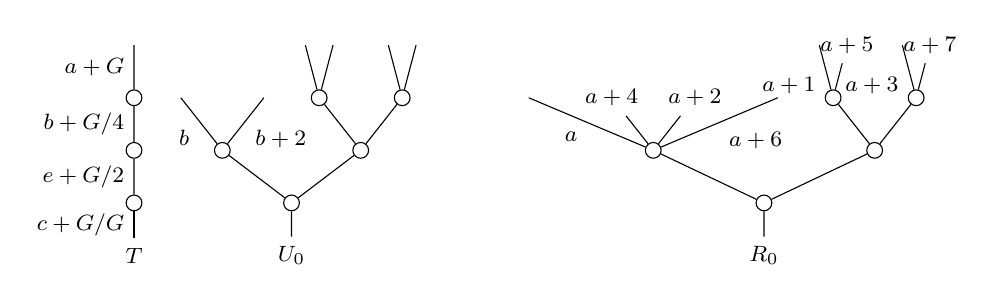
\begin{tikzpicture}[grow=up, every node/.style = {font=\footnotesize},level distance = 1.9em, auto]
                  \tikzstyle{level 2}=[sibling distance=5em]%
                  \tikzstyle{level 3}=[sibling distance=3em]%
                  \tikzstyle{level 4}=[sibling distance=1em]%
                  \node{$T$}
                  child{node [dummy] {}
                    child{node [dummy] {}
                      child{node [dummy] {}
                        child{
                          edge from parent node {$a+G$}
                        }
                        edge from parent node {$b+G/4$}
                      }
                      edge from parent node {$e+G/2$}
                    }
                    edge from parent node {$c+G/G$}
                  };
                  \node at (2,0) {$U_0$}
                  child{node [dummy] {}
                    child{node [dummy] {}
                      child{node [dummy] {}
                        child{}
                        child{}
                      }
                      child{node [dummy] {}
                        child{}
                        child{}
                      }
                    }
                    child{node [dummy] {}
                      child{edge from parent node [swap] {$b+2$}}
                      child{edge from parent node {$b$}}
                    }
                  };
                  \tikzstyle{level 2}=[sibling distance=8em]%
                  \node at (8,0) {$R_0$}
                  child{node [dummy] {}
                    child{node [dummy] {}
                      child{node [dummy] {}
                        child{node {$a+7$}}
                        child{edge from parent node {$a+3$}}
                      }
                      child{node [dummy] {}
                        child{node {$a+5$}}
                        child{edge from parent node {$a+1$}}
                      }
                    }
                    child{node [dummy] {}
                      child{edge from parent node [swap]{$a+6$}}
                      child{node {$a+2$}}
                      child{node {$a+4$}}
                      child{edge from parent node {$a$}}
                    }
                  };
            \end{tikzpicture}
      \end{equation}
      Both $U_0$ and $R_0$ are in $\mathscr{F}^{-o}(T)$, and have actions by $2G$.
      They are also only contained in faces in $\Lambda^{G e}[T]$ which have strictly smaller isotropy,
      meaning they need to be attached themselves, as not as part of a larger face.
      However, both orbital horns $\Lambda^{G e}_o[G \cdot_{2G} U_0]$ and $\Lambda^{G e}_o[G \cdot_{2G} R_0]$
      miss the face $S_0$ below, so it would be attached \textbf{twice} when trying to construct
      $\Lambda^{G e}[T]$ from $\Lambda^{G e}_o[T]$ cellularly.
      \begin{equation}
            \begin{tikzpicture}[grow=up, every node/.style = {font=\footnotesize},level distance = 1.9em, auto]
                  \tikzstyle{level 2}=[sibling distance=5em]%
                  \node {$S_0$}
                  child{node [dummy] {}
                    child{node [dummy] {}
                      child{node [dummy] {}
                        child{}
                        child{}
                      }
                      child[level distance=3em]{node {$a+5$}}
                      child[level distance=3em]{node {$a+1$}}
                    }
                    child{edge from parent node {$e$}}
                  };
            \end{tikzpicture}
      \end{equation}
\end{example}





% \begin{example}[A Problem with the Reverse]
%       With $G = C_4$, consider the tree
%       \begin{equation}
%             \begin{tikzpicture}[grow=up, every node/.style = {font=\footnotesize},level distance = 1.9em, auto]%
%                   \tikzstyle{level 3}=[sibling distance=5.75em]%
%                   \tikzstyle{level 4}=[sibling distance=2em]%
%                   \node {$T$}
%                   child{node [dummy] {}
%                     child{node [dummy] {}
%                       child{node [dummy] {}
%                         child{edge from parent node [swap] {$a+3$}}
%                         child{edge from parent node {$a+1$}}
%                         edge from parent node [swap] {$b+1$}
%                       }
%                       child{node [dummy] {}
%                         child{edge from parent node [swap]{$a+2$}}
%                         child{edge from parent node {$a$}}
%                         edge from parent node {$b$}
%                       }
%                       edge from parent node [swap] {$e$}
%                     }
%                     edge from parent node [swap] {$c$}
%                   };
%             \end{tikzpicture}
%       \end{equation}
%       The map $\Lambda^{G e}[T] \to \Omega[T]$ does not appear to be in the hypersaturation of orbital horn inclusions.
%       In particular, the map itself cannot be built out of orbital horn inclusions (too few missing dendricies),
%       and the map $\Lambda^{G e}_o[T] \to \Lambda^{G e}[T]$
%       does not appear to be cellular on orbital horn inclusions.
% \end{example}




















\subsection{Actual Stuff}

Recall that a class of maps is called \textit{saturated}
if it is closed under pushouts, transfinite composition and retracts.
Moreover, following the discussion preceding \cite[Prop. 3.6.8]{HHM16}, we will call a class of maps of $\mathsf{dSet}^G$ \textit{hypersaturated} if it is further closed under the following cancellation property: if in
\[
A \xrightarrow{f} B \xrightarrow{g} C
\]
both $f$ and $gf$ are in the class, then so is $g$.

The following is an equivariant generalization of 
\cite[Props. 2.4 and 2.5]{CM13a}.

\begin{proposition}\label{HYPER PROP}
The following sets of maps generate the same hypersaturated class:
\begin{itemize}
\item the $G$-inner horn inclusions
$\Lambda^{Ge} [T] \to \Omega[T]$ for $T \in \Omega_G$ and $Ge$ an inner edge orbit; 
\item the orbital $G$-inner horn inclusions
$\Lambda^{Ge}_o [T] \to \Omega[T]$ for $T \in \Omega_G$ and $Ge$ an inner edge orbit; 
\item the $G$-segal core inclusions
$Sc [T] \to \Omega[T]$ for $T \in \Omega_G$.
\end{itemize}
Moreover, one also has the following:
\begin{itemize}
	\item[(a)] orbital $G$-inner horn inclusions are in the saturation of $G$-inner horn inclusions;
	\item[(b)] $G$-segal core inclusions are in the saturation of both orbital $G$-inner horn and $G$-inner horn inclusions.
\end{itemize}
\end{proposition}


\begin{remark}
	Setting $G=e$ and slicing over the stick tree $\eta$ in the previous result
	one recovers the well known claim that 
	the hypersaturation of the simplicial inner horns
	$\{\Lambda^i[n] \to \Delta[n] \colon 0< i < n\}$
	coincides with the hypersaturation of the simplicial Segal core inclusions
	$\{Sc[n] \to \Delta[n]\colon n \geq 2\}$.
\end{remark}


\begin{remark}\label{HYPERSATKAN REM}
	We will also make use of a variant of the previous remark for the hypersaturation of \textit{all} simplicial horns.
	Namely, we claim that the hypersaturation of all simplicial horns 
	$\{\Lambda^i[n] \to \Delta[n] \colon 0 \leq i \leq n\}$
	coincides with the hypersaturation of all vertex inclusion maps
	$\{\Delta[0] \to \Delta[n]\}$.
	Indeed, call the latter hypersaturation $S$. 
	An easy argument shows that the Segal core inclusions 
	$\{Sc[n] \to \Delta[n]\}$ are in $S$ and thus so are all inner horn inclusions. On the other hand, the skeletal filtration of the left horns $\Lambda^0[n]$ is built exclusively out of left horn inclusions, and thus since $\Delta[0]=\Lambda^0[1] \to \Delta[1]$ is in $S$ so are all left horn inclusions 
	$\Lambda^0[n] \to \Delta[n]$. The case of right horn inclusions $\Lambda^n[n] \to \Delta[n]$ is dual.
\end{remark}

\begin{notation}
Given subgroups $H_i \leq G$, $0\leq i \leq k$ such that
$H_0 \geq H_i$, $1 \leq i \leq k$ we write
$C_{\amalg_i H_0/H_i}$ for the $G$-corolla encoding the 
$H_0$-set $H_0/H_1 \amalg \cdots \amalg H_0/H_k$.
\end{notation}


The following is the equivariant generalization of 
\cite[Thm. 3.5]{CM13a}.

\begin{proposition}\label{TFAE PROP}
Let $X \to Y$ be a map between $G$-$\infty$-operads. The following are equivalent:
\begin{enumerate}
	\item[(a)] for all $G$-corollas $C_A$ and $H\leq G$ the maps
\[k(\Omega[C_A],X) \to k(\Omega[C_A],Y), \qquad
k(\Omega[G/H \cdot \eta],X) \to k(\Omega[G/H \cdot \eta],Y)
\]
are weak equivalences in $\mathsf{sSet}$;
	\item[(b)] for all $G$-trees $T$ the maps 
	\[k(\Omega[T],X) \to k(\Omega[T],Y) \]
are weak equivalences in $\mathsf{sSet}$;
	\item[(c)] for all normal $G$-dendroidal sets $A$, the maps
	\[k(A,X) \to k(A,Y) \]
are weak equivalences in $\mathsf{sSet}$;
	\item[(d)] $f \colon X \to Y$ is a weak equivalence in 
	$\mathsf{dSet}^G$.
\end{enumerate}
\end{proposition}


\begin{definition}\label{PROF DEF}
	Let $X$ be a $G$-$\infty$-operad.
	A \textit{$G$-profile} on $X$ is a map
\[
	\partial \Omega[C] \to X
\]
	for some $G$-corolla $C \in \Sigma_G$.

More explicitly, a $G$-profile consists of:
\begin{itemize}
	\item subgroups $H_i \leq G$, $0\leq i \leq k$ such that
	$H_0 \geq H_i$ for $1 \leq i \leq k$;
	\item objects $x_i \in X(\eta)^{H_i}$ for $0 \leq i \leq k$.
\end{itemize}
To simplify notation, we will prefer to denote a $G$-profile as 
$(x_1,\cdots,x_k;x_0)$, and refer to it as a 
\textit{$C$-profile}.
\end{definition}


\begin{definition}\label{MAPSPACE DEF}
Given a $G$-$\infty$-operad and a $C$-profile 
$(x_1,\cdots,x_k;x_0)$ we define the space of maps
$X(x_1,\cdots,x_k;x_0)$ to be given by the pullback
\[
\begin{tikzcd}
	X(x_1,\cdots,x_k;x_0) \ar{r} \ar{d}&
	Hom(\Omega[C],X) \ar{d}
\\
	G \cdot \eta \ar{r}[swap]{(x_1,\cdots,x_k;x_0)} &
	\prod_{0\leq i \leq k} X(\eta)^{H_i}
\end{tikzcd}
\]
Noting that there are equivalences of categories (the first of which is an isomorphism)
\[(\mathsf{dSet}_G) / G\cdot \eta \simeq 
\mathsf{sSet}^{B_G} \simeq \mathsf{sSet},\]
 one sees that 
$X(x_1,\cdots,x_k;x_0)$ 
can indeed be regarded as a simplicial set (in fact, this is a Kan complex).
\end{definition}


\begin{definition}
Let $f \colon X \to Y$ be a map of $G$-$\infty$-operads.

The map $f$ is called \textit{fully faithful} if, for each $C$-profile $(x_1,\cdots, x_k ; x_0)$ one has that
\[
X(x_1,\cdots,x_k;x_0) \to Y\left(f(x_1),\cdots,f(x_k);f(x_0)\right)
\]
is weak equivalence in $\mathsf{sSet}$.

The map $f$ is called \textit{essentially surjective} if for each subgroup $H \leq G$ the map of categories
$\tau(\iota^{\**}(X^H)) \to \tau(\iota^{\**}(Y^H))$
are essentially surjective.
\end{definition}

The following is the equivariant generalization of 
\cite[Thm. 3.11 and Remark 3.12]{CM13a}.


\begin{theorem}
A map $f \colon X \to Y$ of $G$-$\infty$-operads is fully faithful iff for all $G$-corollas $C \in \Sigma_G$ the commutative squares
of Kan complexes
\begin{equation}\label{COMSQ EQ}
\begin{tikzcd}
	k(\Omega[C],X) \ar{r} \ar{d}[swap]{p}&
	k(\Omega[C],Y) \ar{d}{q}
\\
	k(\partial \Omega[C],X) \ar{r}[swap]{f_{\**}} &
	k(\partial \Omega[C],Y)
\end{tikzcd}
\end{equation}
are homotopy pullback squares.

Hence, $f$ is a weak equivalence in $\mathsf{dSet}^G$ iff $f$ is both fully faithful and essentially surjective. 
\end{theorem}

\begin{proof}
Noting that the $0$-simplices of $k(\partial \Omega[C],X)$
are precisely the $C$-profiles $(x_1,\cdots,x_k,x_0)$,
fully faithfulness can be reinterpreted as saying that all fiber maps
$p^{-1}(x_1,\cdots,x_k,x_0) \to 
q^{-1}(f(x_1),\cdots,f(x_k),f(x_0))$
are weak equivalences. But since $p,q$ are Kan fibrations, this is equivalent to the condition that \eqref{COMSQ EQ}
is a homotopy pullback (see \cite[Lemma 3.9]{CM13a}), and the first half follows.

For the second half, note first that the bottom map in 
\eqref{COMSQ EQ} can be rewritten as
\[
	\prod_{0\leq i \leq k} k \left(G/H_i \cdot \eta, X \right) \to 
	\prod_{0\leq i \leq k} k \left(G/H_i \cdot \eta, Y \right).
\]

Assume first that $f$ is a weak equivalence. Proposition \ref{TFAE PROP} then implies that the horizontal maps in \eqref{COMSQ EQ}
are weak equivalences, so that the square is a pull back square, and thus $f$ is fully faithful. 
That $f$ is essentially surjective follows from the identity
$k \left(G/H \cdot \eta, X \right) = k(\iota^{\**}(Z^H))$, so that 
$\tau(\iota^{\**}(X^H)) \to \tau(\iota^{\**}(Y^H))$ is essentially surjective at the level of maximal groupoids, and this suffices for essential surjectivity.

Assume now that $f$ is fully faithful and essentially surjective. Since \eqref{COMSQ EQ}, Proposition \ref{TFAE PROP} now implies that one needs only check that the maps of Kan complexes
\begin{equation}\label{KANMAP EQ}
	k \left(G/H \cdot \eta, X \right) \to 
	k \left(G/H \cdot \eta, Y \right)
\qquad \text{or} \qquad
	k\left(\iota^{\**}\left(X^H\right)\right) \to 
	k\left(\iota^{\**}\left(Y^H\right)\right)
\end{equation}
are weak equivalences. As before, essential surjectivity is equivalent to the fact that the maps \eqref{KANMAP EQ} induce surjections on connected components. Hence, it now suffices to show that for each $0$-simplex $x \in X^H$ the top map of loop spaces in 
\begin{equation}\label{OMEGASQ EQ}
\begin{tikzcd}
	\Omega(k(\iota^{\**}X^H),x) \ar{r} \ar{d} &
	\Omega(k(\iota^{\**}Y^H),f(x)) \ar{d}
\\
	X(x;x) \ar{r} &
	Y(f(x);f(x))
\end{tikzcd}
\end{equation}
is a weak equivalence. Noting that the bottom map in 
\eqref{OMEGASQ EQ}
is a weak equivalence since $F$ is fully faithful
 and that the vertical maps are the inclusion of the connected components corresponding to automorphisms of $x$ in 
 $\tau(\iota^{\**} X^H)$.
 It thus suffices to check that the top map in
 \eqref{OMEGASQ EQ} is an isomorphism on $\pi_0$,
 and this follows since the map of categories
 $\tau(\iota^{\**}(X^H)) \to \tau(\iota^{\**}(Y^H))$
 is fully faithful. 
\end{proof}


\section{Equivariant simplicial dendroidal sets}

The results in \cite[\S 4]{CM13a}
concerning the simplicial Reedy model structure all generalized mutatis mutandis.

\begin{proposition}\label{COMBMODSTR PROP}
	Suppose $\mathcal{C}$
	admits two model structures $(C,W_1,F_1)$ and $(C,W_2,F_2)$
	with the same class of cofibrations, and assume further that both model structures are cofibrantly generated and admit left Bousfield localizations with respect to any set of maps.
	
	Then there is a smallest common left Bousfield localization 
	$(C,W,F)$ and for any $(C,W,F)$-local 
	$c,d$ objects one has that $c\to d$ is in $W$ iff it is in $W_1$ iff it is in $W_2$.
	
	Moreover, an object $X$ is local in the common left Bousfield localization iff it is simultaneously fibrant in both of the two initial model structures.
\end{proposition}

\begin{proof}
	The model structure $(C,W,F)$ can be obtained by either localizing $(C,W_1,F_1)$ with regards to the generating trivial cofibrations of $(C,W_2,F_2)$ or vice-versa. That the two processes yield the same model structure follows from from the universal property of left Bousfield localizations \cite[Prop. 3.4.18]{Hir03}.
	The claim concerning local $c,d$ follows from the local Whitehead theorem \cite[Thm. 3.3.8]{Hir03}, stating that
the local equivalences between local objects match the
initial weak equivalences.

That local objects are fibrant in both model structures follows since $C \cap W$ contains both $C \cap W_1$ and $C\cap W_2$ (in fact, this shows that local fibrations are fibrations in both model structures). The converse claim follows from the observation that fibrant objects in any model structure are local with respect to the weak equivalences in that same model structure.
\end{proof}

The prototypical example of Proposition \ref{COMBMODSTR PROP}
is given by the category $\mathsf{ssSet}$ of bisimplicial sets together with the two possible Reedy structures (over the Kan model structure on $\mathsf{sSet}$).

Explicitly, writing the levels of 
$X \in \mathsf{ssSet}$ as $X_{n,m}$
one can either form a Reedy model structure with respect to the 
\textit{horizontal index $n$}
or with respect to the 
\textit{vertical index $m$}.
In either case, the generating cofibrations are then given by the maps
\[
	\left( \partial \Delta[n] \to \Delta[n] \right)
\square
	\left( \partial \Delta[m] \to \Delta[m] \right),
\qquad n,m\geq 0.
\] 
Further, in the horizontal Reedy model structure the generating trivial cofibrations are the maps
\[
	\left( \partial \Delta[n] \to \Delta[n] \right)
\square
	\left( \Lambda^j[m] \to \Delta[m] \right),
\qquad n\geq 0,m\geq j \geq 0.
\]
while for the vertical Reedy model structure the generating trivial cofibrations are the maps
\[
	\left( \Lambda^i[n] \to \Delta[n] \right)
\square
	\left( \partial \Delta[m] \to \Delta[m] \right),
\qquad n \geq i \geq 0,m\geq 0.
\]
We caution the reader about a possible hiccup with the terminology: 
the weak equivalences for the horizontal Reedy structure are the 
\textit{vertical equivalences},
i.e. maps inducing Kan equivalences of simplicial sets
$X_{n,\bullet} \to Y_{n,\bullet}$
for each $n \geq 0$, and dually for the vertical Reedy structure.

In the next result we refer to the localized model structure given by Proposition \ref{COMBMODSTR PROP} as the 
\textit{joint Reedy model structure}.

\begin{proposition}\label{SSSETJREE PROP}
	Suppose that $X, Y \in \mathsf{ssSet}$ are horizontal Reedy fibrant. Then:
\begin{itemize}
	\item[(i)] for each fixed $m$ all vertex maps $X_{\bullet,m} \to X_{\bullet,0}$ are trivial Kan fibrations;
	\item[(ii)] any vertical Reedy fibrant replacement $\tilde{X}$ of $X$ is in fact fibrant in the joint Reedy model structure;
	\item[(iii)] a map $X \to Y$ is a horizontal weak equivalence iff it is a joint weak equivalence;
	\item[(iv)] the canonical map $X_{n,0} \to X_{n,n}$ is a Kan equivalence.
\end{itemize}
\end{proposition}

\begin{proof}
(i) follows since the trivial cofibrations for the horizontal Reedy structure include all the maps of the form
$(\partial \Delta[n] \to \Delta[n]) \square (\Delta[0] \to \Delta[m])$.

(ii) follows since by (i) $\tilde{X}$ is then local
(with the vertical Reedy model structure as the initial model structure)
with respect to all maps of the form
$\Delta[0] \times (\Delta[0] \to \Delta[m])$,
and thus by Remark \ref{HYPERSATKAN REM}
it is fibrant in the joint Reedy model structure ({\color{blue} add a remark about this}).

(iii) follows from (ii) since the localizing maps 
$X \to \tilde{X}$, $Y \to \tilde{Y}$
are horizontal equivalences.

For (iv), note first that the diagonal functor
$\Delta \colon \mathsf{ssSet} \to \mathsf{sSet}$
is left Quillen for either the horizontal or vertical Reedy structures (and thus also for the joint Reedy structure). But noting that all objects are cofibrant, and regarding 
$X_{n,0}$ as a bisimplicial set that is vertically constant, the claim
follows by noting that by (i) the map
$X_{n_0} \to X$ is a horizontal weak equivalence in $\mathsf{ssSet}$.
\end{proof}

\begin{corollary}
	A map $f\colon X \to Y$ in $\mathsf{ssSet}$ is a joint equivalence iff it induces a Kan equivalence on diagonals
	$\Delta(X) \to \Delta(Y)$ in $\mathsf{sSet}$.
\end{corollary}

\begin{proof}
	Since horizontal Reedy fibrant replacement maps
	$X \to \tilde{X}$ are diagonal equivalences, 
	one reduces to the case of $X,Y$ horizontal Reedy fibrant.
	
	But Proposition \ref{SSSETJREE PROP} (i) and (iii) then combine to say that $X \to Y$ is a joint equivalence iff
	$X_{\bullet,0} \to Y_{\bullet,0}$ is a Kan equivalence, 
	so that the result follows from Proposition \ref{SSSETJREE PROP} (iv).
\end{proof}


We now turn to our main application of Proposition \ref{COMBMODSTR PROP}, the category 
$\mathsf{sdSet}^G = \mathsf{Set}^{\Delta^{op} \times \Omega^{op} \times G}$
of $G$-equivariant simplicial dendroidal sets.

Using the fact that $\Delta$ is a (usual) Reedy category
and the model structure on $\mathsf{dSet}^G$ given by 
\cite[Thm. 2.1]{Per17}
yields a model structure on $\mathsf{sdSet}^G$
that we will refer to as the \textit{simplicial Reedy model structure}.

On the other hand, in the context of Definition \ref{GENRED DEF},
$\Omega^{op} \times G$ is a generalized Reedy category such that the families $\{\mathcal{F}_{U}^{\Gamma}\}_{U \in \Omega}$
of $G$-graph subgroups are Reedy-admissible 
(see Example \ref{GGRAPHREEDY EX}), 
and hence using the underlying 
Kan model structure on $\mathsf{sSet}$, 
Theorem \ref{REEDYADM THM} yields
a model structure on $\mathsf{sdSet}^G$
that we will refer to as the \textit{equivariant dendroidal Reedy model structure}, 
or simply as \textit{dendroidal Reedy model structure} for the sake of brevity.

\begin{proposition}
	Both the simplicial and dendroidal Reedy model structures on 
	$\mathsf{sdSet}^G$ have generating cofibrations given by the maps
\[
	\left(\partial \Delta [n] \to \Delta[n]\right)
		\square
	\left(\partial \Omega[T] \to \Omega[T]\right),
	\qquad
	n\geq 0, T \in \Omega_G.
\]
Further, the dendroidal Reedy structure has generating trivial cofibrations the maps
\begin{equation}\label{DENDTRIVCOF EQ}
	\left(\Lambda^i [n] \to \Delta[n]\right)
		\square
	\left(\partial \Omega[T] \to \Omega[T]\right),
	\qquad
	n\geq i \geq 0, T \in \Omega_G.
\end{equation}
while the simplicial Reedy structure has generating trivial cofibrations the maps
\begin{equation}\label{SIMPTRIVCOF EQ}
	\left(\partial \Delta [n] \to \Delta[n]\right)
		\square
	\left(A \to B\right),
	\qquad
	n\geq 0
\end{equation}
for $\{A \to B\}$ a set of generating trivial cofibrations of
$\mathsf{dSet}^G$.
\end{proposition}

\begin{proof}
	For the claims concerning the dendroidal Reedy structure, 
	note that the presheaves $\Omega[T] \in \mathsf{dSet}^G$
	are precisely the quotients $(G \cdot \Omega[U])/K$ for $U\in \Omega$ and $K \leq G \times \Sigma_U$ a $G$-graph subgroup,
	so that $\partial \Omega[T] \to \Omega[T]$
	represents the maps $X_U^K \to (M_U X)^K$ for $X \in \mathsf{dSet}^G$.
	
	The claims concerning the simplicial Reedy structure are immediate.
\end{proof}


\begin{corollary}\label{JOINTFIBCHAR COR}
The joint fibrant objects $X \in \mathsf{sdSet}^G$ have the following equivalent characterizations:
\begin{itemize}
	\item[(i)] $X$ is both simplicial Reedy fibrant and dendroidal Reedy fibrant;
	\item[(ii)] $X$ is simplicial Reedy fibrant and all maps 
	$X_0 \to X_n$ are equivalences in $\mathsf{dSet}^{G}$;
	\item[(iii)] $X$ is dendroidal Reedy fibrant and all maps
\[
	X^{\Omega[T]} \to X^{Sc[T]}
\qquad \text{and} \qquad
	X^{\Omega[T]} \to X^{\Omega[T]\otimes J_d}
\]
for $T \in \Omega_G$ are Kan equivalences in $\mathsf{sSet}$.
\end{itemize}
\end{corollary}


\begin{proof}
	(i) simply repeats the last part of Proposition \ref{COMBMODSTR PROP}. In the remainder we write $K \to L$ for a generic monomorphism in 
$\mathsf{sSet}$
and $A \to B$ a generic normal monomorphism in $\mathsf{dSet}^G$.

	For (ii), note first that $X$ is simplicial fibrant iff 
$X^L \to X^K$ is always a fibration in $\mathsf{dSet}^G$. 
Hence, such $X$ will have the right lifting property againt all maps in \eqref{DENDTRIVCOF EQ} iff 
$X^L \to X^K$ is a trivial fibration whenever $K \to L$ is anodyne. But Remark \ref{HYPERSATKAN REM}
implies that it suffices to verify this for
the vertex inclusions $\Delta[0] \to \Delta[n]$.

For (iii), note first that $X$ is dendroidal fibrant iff $X^B \to X^A$ is always a Kan fibration in $\mathsf{sSet}$.
Therefore, $X$ will have the right lifting property against all maps \eqref{SIMPTRIVCOF EQ} iff 
$X^B \to X^A$ is a trivial Kan fibration whenever $A\to B$ is a generating trivial of $\mathsf{dSet}^G$.
By adjunction, this is equivalent to showing that
$X^L \to X^K$ is a fibration in $\mathsf{dSet}^G$ for any monomorphism $K \to L$ in $\mathsf{sSet}$. Moreover, by the fibration between fibrant objects part of \cite[Prop. 8.8]{Per17}
(see also the beginning of \cite[\S 8.1]{Per17})
it suffices to verify that the maps $X^L \to X^K$ have the right lifting property against the maps
\[
	\Lambda^{G e} \Omega[T] \to \Omega[T],
	\quad
	T \in \Omega_G, e \in Inn(T)
\qquad
\text{and}
\qquad
	\Omega[T] \otimes \left( \{i\} \to J_d\right),
	\quad
	T \in \Omega_G, i = \{0,1\}
\]
and it thus suffices to check that $X^B \to X^A$ is a trivial Kan fibration whenever $A\to B$ is one of these maps.
Proposition \ref{HYPER PROP} now finishes the proof.
\end{proof}

We now obtain the following partial analogue of Proposition \ref{SSSETJREE PROP}. Note that the equivalences in the simplicial Reedy model structure are the dendroidal equivalences and vice versa.

\begin{corollary}\label{SDSETG COR}
	Suppose that $X, Y \in \mathsf{sdSet}^G$ are dendroidal Reedy fibrant. Then:
\begin{itemize}
	\item[(i)] for each fixed $m$ all vertex maps $X_{\bullet,m} \to X_{\bullet,0}$ are trivial fibrations in $\mathsf{dSet}^G$;
	\item[(ii)] any simplicial Reedy fibrant replacement $\tilde{X}$ of $X$ is in fact fibrant in the joint Reedy model structure;
	\item[(iii)] a map $X \to Y$ is a dendroidal weak equivalence iff it is a joint weak equivalence;
	\item[(iv)] regarding $X_0$ as a simplicially constant object in $\mathsf{sdSet}^G$, the map $X_0 \to X$ is a dendroidal equivalence, and thus a joint equivalence. (iv) follows from (i).
\end{itemize}
\end{corollary}

\begin{proof}
	The proof adapts that of Proposition \ref{SSSETJREE PROP}.
	(i) follows since $X$ then has the right lifting property with respect to all maps 
	$(\Delta[0] \to \Delta[m]) \square (\partial \Omega[T] \to \Omega[T])$. (ii) follows from (i) and the characterization in  Corollary \ref{JOINTFIBCHAR COR} (ii). (iii) follows from (ii) since the simplicial fibrant replacement maps 
	$X \to \tilde{X}$ are dendroidal equivalences.
\end{proof}


\begin{theorem}
	The inclusion/$0$-th level adjunction
	\[
	\iota\colon 
	\mathsf{dSet}^G \rightleftarrows \mathsf{sdSet}^G
	\colon (-)_0,
	\]
	where $\mathsf{sdSet}^G$ is given the joint Reedy model structure,
	is a Quillen equivalence.
\end{theorem}

\begin{proof}
	It is clear that the inclusion preserves both normal monomorphisms and all weak equivalences, hence the adjunction is Quillen. 
	Consider any map $\iota(A) \to X$ with $X$ joint fibrant and perform a trivial cofibration followed by fibration factorization on the left
\[
\iota(A) \xrightarrow{\sim} \widetilde{\iota(A)} \to X
	\qquad
A \xrightarrow{\sim} \widetilde{\iota(A)}_0 \to X_0
\]
	for the simplicial Reedy model structure. 
	Corollary \ref{JOINTFIBCHAR COR} (ii) now implies that 
	$\widetilde{\iota(A)}$ is in fact joint fibrant
	and thus that the leftmost composite above is a joint equivalence iff $\widetilde{\iota(A)} \to X$ is a dendroidal equivalence in $\mathsf{sdSet}^G$ iff $\widetilde{\iota(A)}_0 \to X_0$ is an equivalence in  $\mathsf{dSet}^G$ iff the rightmost composite is an equivalence in $\mathsf{dSet}^G$.
\end{proof}


\begin{remark}\label{CONCRECOM REM}
	Given a $G$-$\infty$-operad $X$, a joint fibrant model in 
	$\mathsf{sdSet}^G$ is given by 
	$X^{J_d(m)}$.
	Moreover, note that it follows from 
	\cite[Cor. 8.21]{Per17}
	that $u_{\**}(X^{J_d(m)}) = X^{(J_d(m))} \to X^{(\Delta_m)}$
	is a trivial fibration in $\mathsf{sdSet_G}$, 
	so that $X^{J_d(m)}(T) \sim k(\Omega[T],X)$.
\end{remark}

\section{Pre-operads}

Recall that the category $\mathsf{PreOp}$
of \textit{pre-operads} is the full subcategory
$\mathsf{PreOp} \subset \mathsf{sdSet}$
of those $X$ such that $X(\eta)$ is a discrete simplicial set.
Writing $\gamma^{\**}$ for the inclusion one has left and right adjoints $\gamma_!$ and $\gamma_{\**}$
\begin{equation}
\begin{tikzcd}[column sep =5em]
	\mathsf{PreOp}^G \ar{r}[swap]{\gamma^{\**}} 
	&
	\mathsf{sdSet}^G
	\ar[bend right]{l}[swap,midway]{\gamma_{!}}
	\ar[bend left]{l}{\gamma_{\**}}
\end{tikzcd}
\end{equation}
described as follows \cite[\S 7]{CM13a}:
$\gamma_{!}X (T) = X(T)$ if $T \not \in \Delta$
while $\gamma_{!}X ([n])$ for $[n] \in \Delta$ is given by the pushout on the left below; 
$\gamma_{\**}X(T)$ is given by the pullback on the right below.
\[
\begin{tikzcd}
	X(\eta) \ar{r} \ar{d} \arrow[dr, phantom, "\ulcorner", very near start]  &
	\pi_0 X(\eta) \ar{d}
&& 
	\gamma_{\**}X(T) \ar{r} \ar{d} & X(T) \ar{d}
\\
	X([n]) \ar{r} & \gamma_! X([n]) 
&&
	\coprod_{Edges(T)} X(\eta)_0 \ar{r} &
	\coprod_{Edges(T)} X(\eta)
	\arrow[lu, phantom, "\lrcorner", very near start]
\end{tikzcd}
\]


\begin{remark}
	Let $A \to B$ denote a monomorphism in $\mathsf{sdSet}^G$ of the form
\begin{equation}\label{BOUNDRED EQ}
	\left( \partial \Delta[n] \to \Delta [n] \right)
\square
	\left( \partial \Omega[T] \to \Omega [T] \right),
\qquad
	n\geq 0, T\in \Omega_G, T \not = G/H \cdot \eta.
\end{equation}
Then one has an isomorphism $A(\eta) \simeq B(\eta)$
so that the square below is a pushout square.
\begin{equation}\label{GAMMASH EQ}
\begin{tikzcd}
	A \ar{r} \ar{d} \arrow[dr, phantom, "\ulcorner", very near start]&
	\gamma_! A \ar{d}
\\
	B \ar{r} & \gamma_! B 
\end{tikzcd}
\end{equation}
\end{remark}

In the next results we write $I'$ for the set of maps in \eqref{BOUNDRED EQ}.


\begin{lemma}\label{GENSET LEM}
	The normal monomorphisms of $\mathsf{PreOp}^G$ are the saturation of the set of maps
$\{\emptyset \to G/H\cdot \eta | H \leq G\} \cup \gamma_! (I')$.
\end{lemma}


\begin{proof}
	Using the cellular filtration in $\mathsf{sdSet}^G$, 
	any monomorphism $A \to B$ in $\mathsf{PreOp}^G$ can be written as a transfinite composition of pushouts of maps in 
	$\{\emptyset \to G/H\cdot \eta\} \cup I'$.
	But, since the squares \eqref{GAMMASH EQ} are pushouts, the same also holds for the maps 
	$\{\emptyset \to G/H\cdot \eta\} \cup \gamma_!(I')$.
\end{proof}


\begin{lemma}\label{TRIVFIB LEM}
	Any map in $\mathsf{PreOp}^G$ which has the right lifting property against all normal monomorphisms in $\mathsf{PreOp}^G$
	is a joint equivalence in $\mathsf{sdSet}^G$.
\end{lemma}

\begin{proof}
We need simply adapt the proof of \cite[Lemma 8.12]{CM13a} mutatis mutandis. 

Choose a normalization $E_{\infty}$ of $\**$ in 
$\mathsf{sdSet}^G$, i.e. a normal object such that 
$E_{\infty} \to \**$ is a trivial fibration. 
Regarding $E_{\infty}$ as a simplicially constant object in $\mathsf{sdSet}^G$, a map $X\to Y$ in $\mathsf{PreOp}^G$ will have the right lifting property against all monomorphisms iff so does 
$E_{\infty}\times (X\to Y)$, so that one is free to assume $X,Y$ are normal.

One is thus free to pick a section $s\colon Y \to X$
of $p\colon X\to Y$ and regarding $J_d \in \mathsf{dSet}^G$ as a simplicially constant object of $\mathsf{sdSet}^G$ our assumption yields the lift below, so that $p$ is a homotopy equivalence.
\begin{equation}
\begin{tikzcd}[column sep = 4em]
	X \coprod X \ar{r}{(id_X,sp)} \ar{d} &
	X \ar{d}{p}
\\
	X \otimes J_d \ar[dashed]{ru} \ar{r} & Y
\end{tikzcd}
\end{equation}
\end{proof}



\begin{theorem}
	The category $\mathsf{Preop}^G$ of $G$-preoperads has a model structure such that
	\begin{itemize}
		\item the cofibrations are the normal monomorphisms;
		\item the weak equivalences are the maps 
		that become joint equivalences when regarded as maps on 
		$\mathsf{sdSet}^G$.
	\end{itemize}
\end{theorem}

\begin{proof}
One repeats the proof of the non-equivariant analogue \cite[Thm. 8.13]{CM13a}, applying J. Smith's theorem \cite[Thm. 1.7]{Bek00} with the required set of generating cofibrations the 
set $\{\emptyset \to G/H\cdot \eta | H \leq G\} \cup \gamma_! (I')$ given by Lemma \ref{GENSET LEM}.
Indeed, conditions c0 and c2 in \cite{Bek00} are inherited from 
$\mathsf{sdSet}^G$ and c1 follows from Lemma \ref{TRIVFIB LEM}.
The technical ``solution set'' condition c3 follows from 
\cite[Prop. 1.15]{Bek00} since weak equivalences are accessible, being the preimage by $\gamma^{\**}$ of the weak equivalences in 
$\mathsf{sdSet}^G$ 
(see \cite[Cor. A.2.6.5]{Lur09} and \cite[Cor. A.2.6.6]{Lur09}). 
\end{proof}


\begin{theorem}\label{ANOQUEQUIV THM}
	The adjunction
\[
	\gamma^{\**} \colon \mathsf{PreOp}^G	
\rightleftarrows
	\mathsf{sdSet}^G \colon \gamma_{\**}
\]
is a Quillen equivalence.
\end{theorem}

\begin{proof}
	It it tautological that the left adjoint $\gamma^{\**}$
	preserves and detects cofibrations and weak equivalences, so it suffices to show that for all fibrant $X \in \mathsf{sdSet}^G$ there exists $Y \in \mathsf{PreOp}^G$ and a weak equivalence
	$\gamma^{\**}Y \to X$.
	But by Corollary \ref{SDSETG COR} it suffices to take $Y=X_0$, regarded as a simplicially trivial object.
\end{proof}


We will find it useful to also have a characterization of the
fibrant objects in $\mathsf{PreOp}^G$.
In doing so, it becomes useful to consider a fourth model structure on the category $\mathsf{sdSet}^G$ whose fibrant objects ``interpolate'' between the fibrant objects in the two model structures in Theorem \ref{ANOQUEQUIV THM}.
This is the model structure of equivariant dendroidal Segal spaces, that we discuss in the next section.



\section{Equivariant dendroidal Segal spaces}


\begin{definition}
	The \textit{equivariant Segal space model structure} on the category $\mathsf{sdSet}^G$, which we denote 
	$\mathsf{sdSet}^G_S$, 
	is the left Bousfield localization of the dendroidal Reedy model structure with respect to the equivariant Segal core inclusions
\[
	Sc[T] \to \Omega[T], \qquad T \in \Omega_G.
\]
\end{definition}

\begin{remark}
	By Proposition \ref{HYPER PROP} this model structure can equivalently be obtained by localizing with respect to the $G$-inner horn inclusions $\Lambda^{Ge}[T] \to \Omega[T]$.
\end{remark}

\begin{notation}
We will refer to the fibrant objects in 
$\mathsf{sdSet}^G_S$
as \textit{equivariant dendroidal Segal spaces}, 
or just \textit{dendroidal Segal spaces}.
Further, a pre-operad $X \in \mathsf{PreOp}^G$ is called \textit{fibrant}
if $\gamma^{\**}X$ is a dendroidal Segal space.
\end{notation}

\begin{remark}
If $X \in \mathsf{sdSet}^G$ is a dendroidal Segal space, then
$\gamma_{\**}X \in \mathsf{PreOp}^G$ is fibrant. Indeed, the equality $Sc[T](\eta)=\Omega[T](\eta)$ implies that the square below is a pullback square.
\[
\begin{tikzcd}
	\gamma_{\**}X(T) \ar{r} \ar{d} & X(T) \ar{d}
\\
	\left(\gamma_{\**}X\right)^{Sc[T]} \ar{r} &
	X^{Sc[T]}
	\arrow[lu, phantom, "\lrcorner", very near start]
\end{tikzcd}
\]
\end{remark}



The following is a variation on Definition \ref{MAPSPACE DEF}

\begin{definition}\label{MAPSPACESEG DEF}
Given a dendroidal Segal space $X \in \mathsf{sdSet}^G_S$
and a $C$-profile $(x_1,\cdots,x_n ; x_0)$
on $X$ (defined exactly as in Definition \ref{PROF DEF})
we define the space of maps 
$X(x_1,\cdots,x_n ; x_0)$ via the pullback
\[
\begin{tikzcd}
	X(x_1,\cdots,x_k;x_0) \ar{r} \ar{d}&
	X(C) \ar{d}
\\
	G \cdot \eta \ar{r}[swap]{(x_1,\cdots,x_k;x_0)} &
	\prod_{0\leq i \leq k} X(\eta)^{H_i}
\end{tikzcd}
\]
\end{definition}

\begin{definition}
	Let $X \in \mathsf{sdSet}^G$ be a dendroidal Segal space.
	The \textit{homotopy genuine operad} 
	$ho(X)\in \mathsf{dSet_G}$ is defined by
	\[
	ho(X) = \pi_0 \left( u_{\**} \left( \gamma_{\**}X \right) \right).
	\]
\end{definition}

\begin{remark}
	It is immediate that 
	$X(x_1,\cdots,x_k;x_0) = \gamma_{\**}X(x_1,\cdots,x_k;x_0)$, so that both of the previous definitions depend only on 
	the fibrant pre-operad $\gamma_{\**}X$.
\end{remark}

\begin{remark}
It is important not to confuse Definitions \ref{MAPSPACE DEF} 
and \ref{MAPSPACESEG DEF}. Indeed, when $X$ is a dendroidal Segal, its $0$-th level $X_0$ is a $G$-$\infty$-operad, and one can thus form two ``spaces of maps'' 
$X_0(x_1,\cdots,x_k;x_0)$ (cf. Definition \ref{MAPSPACE DEF})
and
$X(x_1,\cdots,x_k;x_0)$ (cf. Definition \ref{MAPSPACESEG DEF}).
The constructions leading to these spaces are quite different. When $X$ is complete Segal, 
the fact that these two spaces are homotopic follows 
from Remark \ref{CONCRECOM REM}, since $X$ must then be both dendroidally and simplicially equivalent to $X_0^{J_d(m)}$. 
The claim that this holds without completeness is harder, with the rest of the section devoted to establishing this.
\end{remark}


\begin{remark}
	Writing $\iota$ for the inclusion $\Delta \to \Omega$
	and $\iota_G$ for the composite inclusion
	$\Delta \times \mathsf{O}_G \to 
	\Omega \times \mathsf{O}_G \to
	\Omega_G$,
	one has that $\iota_G^{\**}ho(X)$ is the $G$-coefficient system of categories formed by the homotopy categories
	$ho \left(\iota^{\**}\left(X^H\right)\right) = 
	\pi_0 \left(\iota^{\**} \gamma_{\**}X^H\right)$.
\end{remark}

\begin{definition}
	A map $f \colon X \to Y$ of equivariant dendroidal Segal spaces is called 
\begin{itemize}
	\item \textit{fully faithful} is for all $C\in \Sigma_G$ and $C$-profile $(x_1,\cdots,x_n;x_0)$ on $X$ the map
\[
	X(x_1,\cdots,x_k;x_0) \to
	Y\left(f(x_1),\cdots,f(x_k);f(x_0)\right)
\]
is a Kan equivalence in $\mathsf{sSet}$;
	\item \textit{essentially surjective} if
	the map $\iota_G^{\**}ho(X) \to \iota_G^{\**}ho(Y)$
	is essentially surjective on all category levels of the $G$-coefficient system;
	\item a \textit{DK-equivalence}\footnote{Here DK stands for Dwyer and Kan.} if it is both fully faithful and essentially surjective.
\end{itemize}
\end{definition}

\begin{remark}
This definition depends only on the map
$\gamma_{\**} X \to \gamma_{\**} Y$
of fibrant pre-operads.
\end{remark}

DK-equivalences will provide an explicit description of complete/joint equivalences between dendroidal Segal objects (and thus also between fibrant pre-operads), as we will prove in
{\color{red} whatever below}. We now introduce some auxiliary notions.

Suppose $C,D \in \Sigma_G$ are $G$-corollas that can be grafted,
i.e. that $C$ has a leaf orbit and $D$ a root orbit both isomorphic to $G/H$. Denote this orbit as $G e$
and write $T= C \amalg_{G e} D$ for the grafted $G$-tree. 
For any dendroidal Segal space $X$ one then has
$X^{Sc[T]} \simeq X(C) \times_{X(\eta)^H} X(D)$
and one can hence form the section in the middle row below
\begin{equation}\label{HOMOTCIRC EQ}
\begin{tikzcd}
	\{\varphi\} \times X(z_1,\cdots,z_l;e)
	\ar[dashed]{rr}{\varphi \circ_{Ge} (-)}
&&
	X(z_1,\cdots,z_l,y_2,\cdots,y_k;x)
\\
	X(C) \times_{X(\eta)^H} X(D) \ar[bend left=17,dashed]{r}
	\ar[hookleftarrow]{u}
&
	X(T) \ar[->>]{l}{\sim} \ar[->>]{r}
&
	X(T-Ge)
	\ar[hookleftarrow]{u}
\\
	X(e,y_2,\cdots,y_k;x) \times \{\psi\}
	\ar[hookrightarrow]{u}
	\ar[dashed]{rr}[swap]{(-)\circ_{Ge} \psi}
&&
	X(z_1,\cdots,z_l,y_2,\cdots,y_k;x)
	\ar[hookrightarrow]{u}
\end{tikzcd}
\end{equation}
thus defining maps 
$\varphi \circ_{Ge} (-)$ (resp. $(-)\circ_{Ge} \psi$)
for any choice of
$\varphi \in X(e,y_2,\cdots,y_k;x)$
(resp. $\psi \in X(z_1,\cdots,z_l;e)$).

\begin{proposition}
	The maps $\varphi \circ_{Ge} (-)$, $(-)\circ_{Ge} \psi$
are well defined up to homotopy. Further, if 
$\varphi,\bar{\varphi} \in X(e,y_2,\cdots,y_k;x)$ are homotopic 
(i.e. in the same connected component), then 
the maps $\varphi \circ_{Ge} (-)$, $\bar{\varphi} \circ_{Ge} (-)$
	are homotopic, and likewise for $\psi$.
	
	In particular, $\varphi \circ_{Ge} \psi \in X(z_1,\cdots,z_l,y_2,\cdots,y_k;x)$
	is well defined up to homotopy.
\end{proposition}

\begin{proof}
	This is immediate once one notes that, writing $E = T-Ge$ for the ``composite $G$-corolla'', all solid maps in 
	\eqref{HOMOTCIRC EQ} are compatible with the projections
	to $X^{\partial \Omega[E]}$.
\end{proof}

	We will now show that the operations   
	$\varphi \circ_{Ge} (-)$, $(-)\circ_{Ge} \psi$
	satisfy the obvious compatibilities one expects, but we will find it convenient to first package these compatibilities into a common format. In the categorical case (corresponding to linear trees), there are three types of compatibilities, corresponding to homotopies
\[
	\varphi \circ \left( \psi \circ (-) \right)
		\sim
	(\varphi \circ \psi) \circ (-) 
\qquad
	\varphi \circ \left( (-)  \circ \psi \right)
		\sim
	\left( \varphi \circ (-) \right) \circ \psi 
\qquad
	\left( (-) \circ \varphi \right) \circ \psi 
		\sim
	(-) \circ (\varphi \circ \psi) 
\]	
but in the operadic case there are instead five cases, corresponding to the different possible roles of the nodes in 
$G$-trees with exactly three $G$-nodes, whose \textit{orbital} representation falls into one of the two cases illustrated below.
\[%
	\begin{tikzpicture}[grow=up, every node/.style = {font=\footnotesize}]%
	\begin{scope}[level distance = 1.9em]
	\tikzstyle{level 2}=[sibling distance=3em]%
	\tikzstyle{level 3}=[sibling distance=1.25em]%
		\node at (5.5,0) {}%
			child{node [dummy] {}%
				child{node {}}%
				child{node [dummy] {}%
					child{}%
					child{}%
					child{}%
				}%
				child{node {}}%
				child{node [dummy] {}%
					child{}%
					child{}%
				}%
			};%
	\end{scope}
	\begin{scope}[level distance = 1.425em]
	\tikzstyle{level 2}=[sibling distance=4em]%
	\tikzstyle{level 3}=[sibling distance=1.5em]%
	\tikzstyle{level 4}=[sibling distance=1em]%
		\node at (0,0) {}%
			child{node [dummy] {}%
				child{node {}}%
				child{node [dummy] {}%
					child{}%
					child{node [dummy] {}
						child
						child}%
					child{}%
					child{}%
				}%
				child{node {}}%
			};%
	\end{scope}
	\end{tikzpicture}%
\]%
Since all these compatibilities can be simultaneously encoded in terms of such trees, we will simply refer to all types of compatibility as ``associativity''.

In the next result, note that a $G$-tree $T$ with three $G$-nodes contains precisely two inner edge orbits $Ge$ and $Gf$. We will write $T[Ge]$ (resp. $T[Gf]$) for the unique orbital outer face of $T$ with $Ge$ (resp. $Gf$) has its single inner edge orbit. 

\begin{proposition}
	The operations   
	$\varphi \circ_{Ge} (-)$, $(-)\circ_{Ge} \psi$
	satisfy all associativity conditions with respect to 
	$3$-nodal $G$-trees.
\end{proposition}

\begin{proof}
	For any $3$-nodal $G$-tree $T$ with inner edge orbits $Ge$, $Gf$, consider the following diagram, 
	where all solid maps are fibrations, and the maps labelled $\sim$ are trivial fibrations.
\begin{equation}\label{FOURSQ EQ}
\begin{tikzcd}[column sep =3.5em,row sep =3.5em]
	X^{\mathsf{Sc}[T]} 
	\ar[bend left=17,dashed]{r}
	\ar[bend right=30,dashed]{d}&
	X^{\mathsf{Sc}_{T[Ge]}[T]}
	 \ar[->>]{l}{\sim} \ar[->>]{r} 
	\ar[bend right=30,dashed]{d}&
	X^{\mathsf{Sc}[T-Ge]}
	\ar[bend right=30,dashed]{d}
\\
	X^{\mathsf{Sc}_{T[Gf]}[T]} \ar[->>]{u}[swap]{\sim} \ar[->>]{d}
	\ar[bend left=17,dashed]{r}& 
	X^{\Omega[T]} \ar[->>]{l}{\sim} \ar[->>]{u}[swap]{\sim} \ar[->>]{r} 
	\ar[->>]{d}&
	X^{\Omega[T-Ge]} \ar[->>]{u}[swap]{\sim} \ar[->>]{d}
\\
	X^{\mathsf{Sc}[T-Gf]} 
	\ar[bend left=17,dashed]{r}&
	X^{\Omega[T-Gf]} \ar[->>]{r} \ar[->>]{l}{\sim}&
	X^{\Omega[T-Ge-Gf]}
\end{tikzcd}
\end{equation}
Noting that the following three diagrams,
where $\Lambda_o^{Ge,Gf}[T]$ is a generalized orbital $G$-horn
and $\Lambda_{o,c}^{Ge}[T]$, $\Lambda_{o,c}^{Gf}[T]$
are characteristic orbital $G$-horns (cf. {\color{red} ref}), are pullbacks
\[
\begin{tikzcd}[column sep =12]
	X^{\mathsf{Sc}[T]} 
	\arrow[rd, phantom, "\ulcorner", near start]& 
	X^{\mathsf{Sc}_{T[Ge]}[T]}
	\ar[->>]{l}{\sim}
&
	X^{\mathsf{Sc}_{T[Ge]}[T]}
	\ar[->>]{r} &
	X^{\mathsf{Sc}[T-Ge]}
	\arrow[ld, phantom, "\urcorner", near start]
&
	X^{\mathsf{Sc}_{T[Gf]}[T]}   \ar[->>]{d}
	& 
	X^{\Lambda_{o,c}^{Ge}[T]} \ar[->>]{l}{\sim}  \ar[->>]{d}
\\
	X^{\mathsf{Sc}_{T[Gf]}[T]} \ar[->>]{u}[swap]{\sim} &
	X^{\Lambda_o^{Ge,Gf}[T]} \ar[->>]{u}[swap]{\sim}
	\ar[->>]{l}{\sim}
&
	X^{\Lambda_{o,c}^{Gf}[T]} \ar[->>]{u}[swap]{\sim}
	\ar[->>]{r} &
	X^{\Omega[T-Ge]} \ar[->>]{u}[swap]{\sim}
&
	X^{\mathsf{Sc}[T-Gf]} 
	\arrow[ur, phantom, "\llcorner", near start]
	&
	X^{\Omega[T-Gf]} \ar[->>]{l}{\sim}&
\end{tikzcd}
\]
one sees that:
\begin{inparaenum}
	\item[(i)] sections in the top left square of \eqref{FOURSQ EQ} can be chosen to be compatible in the sense that the two composites
$X^{Sc[T]} \to X^{\Omega[T]}$ coincide;
	\item[(ii)] 
	sections in the top right and bottom left squares of \eqref{FOURSQ EQ} can be chosen to be compatible in the sense that the two composites
$X^{Sc[T-Ge]} \to X^{\Omega[T]}$ and $X^{Sc[T-Gf]} \to X^{\Omega[T]}$ coincide.
\end{inparaenum}
Note that we do not claim (or need) that (i) and (ii) hold simultaneously.
We thus conclude that the possible choices of maps 
$X^{\mathsf{Sc}[T]} \to X^{\Omega[T-Ge-Gf]}$
given by outer paths in \eqref{FOURSQ EQ}
are homotopic. All desired forms of associativity follow from taking fibers of these maps over the objects $X^{\partial \Omega[T-Ge-Gf]}$.
\end{proof}



\begin{remark}
	While in the non-equivariant case the associativity conditions in the previous result capture all the key compatibilities of the
	$\varphi \circ_{e} (-)$, $(-)\circ_{e} \psi$
	operations, 
	in the equivariant case there are further 
	``compatibilities with pullback of $G$-trees'', which are closely related to the genuine equivariant operads introduced in \cite{BP17}. 
	However, describing these extra compatibilities would require using $G$-trees with more than $3$ $G$-nodes, and since such compatibilites are not needed for our current goals, 
	we omit their discussion. 
\end{remark}

	
	{\color{red} HERE}



\cite{Rez01}

\begin{proposition}
	Let $X\in \mathsf{sdSet}^G$ be a dendroidal Segal space. 
	Then the map $X \to X^{J_d}$ is a $DK$-equivalence.
\end{proposition}

{\color{red} HERE}


\[
	u^{\**} \colon \mathsf{dSet}_G 
\rightleftarrows 
	\mathsf{dSet}^G \colon u_{\**}
\]



{\color{red} discuss characteristic horns}


\newpage


\section{Scratchwork (to be folded into previous sections eventually)}


\begin{lemma}
	One can always form the completion of a dendroidal Segal space $X$ while preserving $X(\eta)_0$. 
\end{lemma}



\begin{proposition}
	A map of $X \to Y$ of dendroidal Segal spaces is a joint equivalence iff it is fully faithful and essentially surjective.
\end{proposition}


\begin{corollary}
	A pre-operad $X \in \mathsf{PreOp}^G$ is fibrant iff $\gamma^{\**}(X)$ is fibrant in the Segal space model structure on 
	$\mathsf{sdSet}^G$.
\end{corollary}


\begin{remark}
The smallest hypersaturated class containing the inner horns and the left horn inclusion
$\Lambda^0[2] \to \Delta[2]$
in fact contains all left horn inclusions
$\Lambda^0[n] \to \Delta[n]$ for $n \geq 2$.
Indeed, this follows inductively from the following diagram since
the bottom map is inner
\begin{equation}
\begin{tikzcd}
	\Lambda^{0,1}[n] \ar{r} \ar{d} &
	\Lambda^{0}[n] \ar{d}
\\
	\Lambda^{1}[n] \ar{r} & \Delta[n] 
\end{tikzcd}
\end{equation}
and the top and left maps are given by following pushouts
\begin{equation}
\begin{tikzcd}
	\Lambda^{0}[n-1] \ar{r} \ar{d} \arrow[dr, phantom, "\ulcorner", very near start]&
	\Lambda^{0,1}[n] \ar{d}
&
	\Lambda^{0}[n-1] \ar{r} \ar{d} \arrow[dr, phantom, "\ulcorner", very near start]&
	\Lambda^{0,1}[n] \ar{d}
\\
	\Delta[n-1] \ar{r}[swap]{d^1} & \Lambda^0[n] 
&
	\Delta[n-1] \ar{r}[swap]{d^0} & \Lambda^1[n] 
\end{tikzcd}
\end{equation}
\end{remark}


\begin{remark}
Write $\widetilde{[n]}$
for the contractible groupoid on objects $\{0,1,\cdots,n\}$. Note that the $k$-simplices of $\widetilde{[n]}$
are encoded as strings $a_0 a_1 \cdots a_k$
with $a_{i} \in \{0,1,\cdots,n\}$, and that a simplex is non-degenerate iff $a_{i-1}\not = a_{i}, 1 \leq i \leq k$.
Then the maps
\begin{equation}\label{INVER EQ}
%	\Delta[2] \xrightarrow{010} N \widetilde{[1]}
%\qquad
	\Delta[n] = N [n] \xrightarrow{012\cdots n} N \widetilde{[n]},\quad n \geq 1
\end{equation}
are built cellularly out of left horn inclusions $\Lambda^{0}[k] \to \Delta[k]$ with $k\geq 2$.

Indeed, we show a little more. Call subcomplex 
$A \subset N \widetilde{[n]}$ is \textit{$0$-stable}
if a $n$-simplex $\underline{a}$ is in $A$ iff the $n+1$-simplex $0\underline{a}$ is.
We claim that any inclusion $A \to A'$ of $0$-stable subcomplexes is built cellularly from left horn inclusions $\Lambda^{0}[k] \to \Delta[k]$ with $k\geq 1$.
Indeed, it suffices to check this when $A'$ attaches as little as 
possible to $A$, and $0$-simplicity guarantees that in that case the only two non-degenerate simplices in $A-A'$
have the form 
$\underline{a}$ and $0\underline{a}$
(note that $\underline{a}$ can not start with a $0$).
But then $A\to A'$ is a pushout of 
$\Lambda^{0}[k+1] \to \Delta[k+1]$ where $k$ is the dimension of $\underline{a}$.

The desired claim follows by noting that both the domain and codomain of \eqref{INVER EQ} are $0$-stable and that the horns 
$\Lambda^0[1]$ are unneeded since \eqref{INVER EQ} is an isomorphism on $0$-simplices.
\end{remark}


\[
\begin{tikzcd}[column sep =3.5em,row sep =3.5em]
	W_1 \times_{W_0} W_1 \times_{W_0} W_1 
	\ar[bend left=17,dashed]{r}
	\ar[bend right=30,dashed]{d}&
	W_1 \times_{W_0} W_2 \ar[->>]{l}{\sim} \ar[->>]{r} 
	\ar[bend right=30,dashed]{d}&
	W_1 \times_{W_0} W_1
	\ar[bend right=30,dashed]{d}
\\
	W_2 \times_{W_0} W_1 \ar[->>]{u}[swap]{\sim} \ar[->>]{d}
	\ar[bend left=17,dashed]{r}& 
	W_3 \ar[->>]{l}{\sim} \ar[->>]{u}[swap]{\sim} \ar[->>]{r} 
	\ar[->>]{d}&
	W_2 \ar[->>]{u}[swap]{\sim} \ar[->>]{d}
\\
	W_1 \times_{W_0} W_1 
	\ar[bend left=17,dashed]{r}&
	W_2 \ar[->>]{r} \ar[->>]{l}{\sim}&
	W_1
\end{tikzcd}
\]

\begin{remark}
	Note that $\mathsf{Sc}_{T[Ge]}$, $\mathsf{Sc}_{T[Gf]}$
	in \eqref{FOURSQ EQ}
	are cover inclusions, and thus $G$-anodyne, relate to 
	\cite[\S 6.2]{Rez10}.
\end{remark}


\begin{remark}
Indexing systems are precisely the Segal sieves of $\Omega_G$.
\end{remark}


\begin{lemma}
	A non-equivariant face $U \hookrightarrow T$ generates an equivariant face $G\cdot U \hookrightarrow T$ iff the $G$-isotropy of $r_U$ matches the isotropy of $U$.
\end{lemma}



%\begin{remark}\label{OUTINP REM}
%	Let $U \hookrightarrow T$ be an outer face.
%	Then for any string of descendancy relations
%	$e <_d e' <_d r$ such that $e,r\in U$ it is also $e' \in U$.
%\end{remark}



\begin{proposition}
	Any non-equivariant face $U \hookrightarrow T$ has a minimal factorization
	$U \hookrightarrow GU \hookrightarrow T$
	through an equivariant face $GU$.
\end{proposition}

\begin{proof}
	Our first task is that of building $GU$. The edges of $GU$ will be given by combining 
	the $G$-orbits of the edges in $U$, but describing the broad relations requires some caution.

	We first assume that $U$ is an outer face and write	$H \leq G$ for the isotropy of the root $r_U$ in $T$.
	We form a (non-equivariant) subtree $HU$ of $T$ with edges (resp. generating broad relations) those edges
	$h u$ (resp. relations $h u^{\uparrow} \leq hu$) in some $hU$ for $h \in H$.
	Indeed, while a priori $HU$ is merely a pre-broad poset of $T$, the antisymmetry and simplicity axioms in \cite[Defs. 5.1 and 5.3]{Per17} are inherited from $T$, and the nodal axiom in
	\cite[Def. 5.9]{Per17} follows since the $h U$, $h \in H$ have a common root. It is now clear that $HU$ inherits a $H$-action and we thus set $GU = G \cdot_H HU$.
	Both the factorization $U \to GU \to T$ and its minimality are immediate from the description of $HU$.
	
	Before tackling the general case, we collect some useful observations. Firstly, the assumption that $U$ is outer implies that so are the (non-equivariant) face $HU$ and the equivariant face $GH$. Secondly, the root tuple of 
	$GU$ is $G\cdot_H r_U$.
	Lastly, we need a characterization of the leaf tuple of $GU$: we call a leaf $l$ of $U$ orbital if 
all the edges in $Hl \cap U$ are leaves of $U$, 
	and claim that the leaves of $GU$ are the tuple $\underline{l}$ formed by the $G$-orbits of the orbital leaves of $U$. Indeed, a leaf $l\in U$ will be a leaf of $HU$ iff whenever $l \in hU$ for some $h\in H$ then $l$ is a leaf of $hU$ iff
	whenever $h^{-1} l \in U$ for some $h\in H$ then $h^{-1}l$ is a leaf of $U$.
	
	In the general case, write $U \to V \to T$ for the factorization
	\cite[Prop. 3.31]{BP17} as a inner face followed by an outer face. 
	We now define $GU$ to be the equivariant inner face of $GV$ that removes all edge orbits that are not represented in $U$
	(that all such edge orbits are inner follows from the description of the roots and leaves of $GV$ in the previous paragraph).
	It is now clear that $U \to GV \to T$ is the minimal factorization with $GV$ an \textit{outer} equivariant face,
	so that the desired factorization $U \to GU \to T$
	follows since inner faces are full while minimality follows
	from the equivariant analogue of the inner face followed by outer face factorization.
%
%	We first assume that $U$ is an outer face and write	$H \leq G$ for the isotropy of the root $r_U$ in $T$.
%	We say that a leaf $l$ of $U$ is orbital if 
%all the edges in $Hl \cap U$ are leaves of $U$, 
%and we write $\underline{l}$ for the tuple formed by the $H$-orbits of the orbital leaves of $U$.
%Note that edges in $\underline{l}$ are $<_d$-incomparable: 
%indeed, whenever it is $l <_d hl' <_d r_V$ with $l,l'$ leaves of $U$
%and $h\in H$ then Remark \ref{OUTINP REM} yields $hl' \in U$, so that $l'$ can not be an orbital leaf.	
%	
%Given $e \in U$, we next write $\underline{l}_e \subseteq \underline{l}$ for the subtuple of those $l$ such that $l \leq_d e$.
%We now make the following key claim:
%for any broad relation $\underline{e} \leq e$ in one of the conjugate trees $hU$ (for $h\in H$) it is 
%$\underline{l}_e \leq \underline{e}$ in $T$.
%The argument is by $\leq_d$ induction on $e$. The base case is that of $e \in \underline{l}$, which holds since $\leq$-incomparability of the edges of $\underline{l}$ then implies
%$\underline{l}_e = e$.
%	Otherwise, there exists some $h \in H$ such that the relation
%	$h e^{\uparrow} \leq he$ is in $hU$ (recall that we are assuming $U$ is outer)
%	and by decomposing the broad relation $h \underline{e} \leq (h e)^{\uparrow}$
%	the induction hypothesis yields
%	$\underline{l}_{h e} \leq h \underline{e}$ and thus also
%	$\underline{l}_e = h^{-1} \underline{l}_{h e} \leq \underline{e}$, as desired.
%	
%	The key claim now yields that $\underline{l} \leq r_U$ and,
%	noting that the relation $\underline{l} \leq r_U$ is $H$-equivariant so that the outer subtree $T_{\underline{l} \leq r_U}$
%	inherits a $H$-action, we define $GU = G \cdot_H T_{\underline{l} \leq r_U}$. 
%	The desired factorization $U \to GU \to T$ is also immediate from the key claim, which further implies that all edges $gu$ and generating relations $gu^{\uparrow}\leq gu$ of the $gU$ are edges and generating relations of $GU$.
%	To check minimality of $GU$, consider any string
%	$u_k <_d u_{k-1} <_d \cdots <_d u_0 = r_U$ in $GU$ where the $\leq_g$ relations are induced by generating $\leq$ relations of $U$. We claim by induction on $k$ that the $u_i$ and generating relations are in some conjugate $g U$. The base case $k=0$ is obvious. Otherwise, by the induction hypothesis it is
%	$u_{k-1} \in gH$ for some $g$, and since it must be  
%	$u_{k-1} \not \in \underline{l}$ (or else $u_k$ it could not be $u_k \in GU$), the relation $g'u_{k-1}^{\uparrow} \leq g' u_{k-1}$ must be in $g'gU$ for some $g' \in G$, and thus minimality of $GU$ follows. 
%	
%	Write $U \to V \to T$ for the factorization
%	\cite[Prop. 3.31]{BP17} as a tall map followed by an outer face
%	as well as $H \leq G$ for the isotropy of the root $r_U=r_V$ in $T$. 
%	We say that a leaf $l$ of $U$ (or, equivalently, of $V$) is orbital if 
%all the edges in $Hl \cap V$ are leaves of $V$.
%
%We now write $\underline{l}$ for the tuple formed by the $H$-orbits of the orbital leaves of $U$.
%Note that edges in $\underline{l}$ are $<_d$-incomparable: 
%indeed, whenever it is $l <_d hl' <_d r_V$ with $l,l'$ leaves of $V$
%and $h\in H$ then Remark \ref{OUTINP REM} yields $hl' \in V$, so that $l'$ can not be an orbital leaf.
\end{proof}

\begin{example}
When $T$ is open then $GU$ is necessarily a full equivariant face, i.e. broad relations coincide with those in $T$, 
and this fact can be leveraged to obtain a simpler proof.

However, the presence of stumps can make the situation 
substantially more subtle, especially in the non-outer case, as illustrated by the following example (where $G = \mathbb{Z}_{/2}=\{\pm1\}$).
\[%
	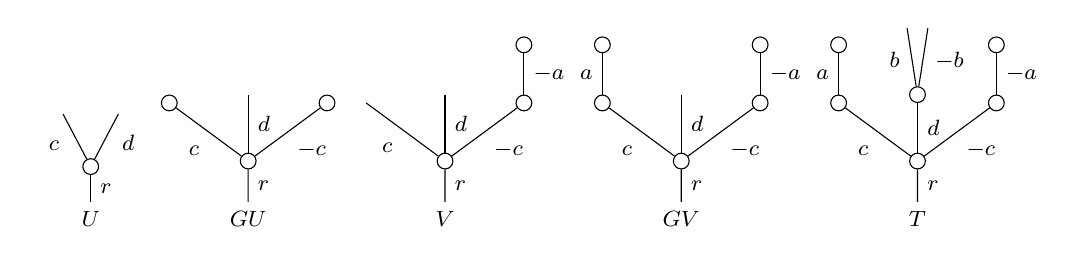
\begin{tikzpicture}[auto,grow=up, every node/.style = {font=\footnotesize}]%
	\begin{scope}[level distance = 1.9em]
	\tikzstyle{level 2}=[sibling distance=2em]%
	\tikzstyle{level 3}=[sibling distance=0.75em]%
		\node at (0,0) {$U$}%
			child{node [dummy] {}%
				child{
				edge from parent node [swap, near end] {$d$}}%
				child{
				edge from parent node [near end] {$\phantom{d}c$}}%
			edge from parent node [swap] {$r$}};%
	\end{scope}
	\begin{scope}[level distance = 2.1em]
	\tikzstyle{level 2}=[sibling distance=2.85em]%
	\tikzstyle{level 3}=[sibling distance=0.75em]%
		\node at (2,0) {$GU$}%
			child{node [dummy] {}%
				child{node [dummy] {}%
				edge from parent node [swap] {$-c$}}%
				child[level distance = 2.4em]{
				edge from parent node [swap] {$d$}}%
				child{node [dummy] {}%
				edge from parent node {$\phantom{-}c$}}%
			edge from parent node [swap] {$r$}};%
		\node at (4.5,0) {$V$}%
			child{node [dummy] {}%
				child{node [dummy] {}%
					child{node [dummy] {}
					edge from parent node [swap] {$-a$}}%
				edge from parent node [swap] {$-c$}}%
				child[level distance = 2.4em]{
				edge from parent node [swap] {$d$}}%
				child{
				edge from parent node {$\phantom{-}c$}}%
			edge from parent node [swap] {$r$}};%
		\node at (7.5,0) {$GV$}%
			child{node [dummy] {}%
				child{node [dummy] {}%
					child{node [dummy] {}
					edge from parent node [swap] {$-a$}}%
				edge from parent node [swap] {$-c$}}%
				child[level distance = 2.4em]{
				edge from parent node [swap] {$d$}}%
				child{node [dummy] {}%
					child{node [dummy] {}
					edge from parent node {$\phantom{-}a$}}%
				edge from parent node {$\phantom{-}c$}}%
			edge from parent node [swap] {$r$}};%
		\node at (10.5,0) {$T$}%
			child{node [dummy] {}%
				child{node [dummy] {}%
					child{node [dummy] {}
					edge from parent node [swap] {$-a$}}%
				edge from parent node [swap] {$-c$}}%
				child[level distance = 2.4em]{node [dummy] {}%
					child{
					edge from parent node [near end,swap]{$-b$}}%
					child{
					edge from parent node [near end]{$\phantom{-}b$}}%
				edge from parent node [swap] {$d$}}%
				child{node [dummy] {}%
					child{node [dummy] {}
					edge from parent node {$\phantom{-}a$}}%
				edge from parent node {$\phantom{-}c$}}%
			edge from parent node [swap] {$r$}};%
	\end{scope}
	\end{tikzpicture}%
\]%

\end{example}



\newpage

\appendix

\section{Equivariant Reedy model structures}

In \cite{BM11} Berger and Moerdijk extend the notion of Reedy category so as to allow for categories $\mathbb{R}$
 with non-trivial automorphism groups 
 $\mathsf{Aut}(r)$ for $r \in \mathbb{R}$.
For such $\mathbb{R}$ and suitable model category $\mathcal{C}$ they then show that there is a 
\textit{Reedy model structure}
on $\mathcal{C}^{\mathbb{R}}$
that is defined by modifying the usual characterizations of
Reedy cofibrations, weak equivalences and fibrations
(see \cite[Thm. 1.6]{BM11} or
Theorem \ref{REEDYADM THM} below)
 to be determined by the $\mathsf{Aut}(r)$-projective model structures
on $\mathcal{C}^{\mathsf{Aut}(r)}$
for each $r \in \mathbb{R}$. 

The purpose of this appendix is to show that,
under suitable conditions, this can also be done by replacing
the $\mathsf{Aut}(r)$-projective model structures
on $\mathcal{C}^{\mathsf{Aut}(r)}$
with the more general 
$\mathcal{C}^{\mathsf{Aut}(r)}_{\mathcal{F}_r}$
model structures for 
$\{\mathcal{F}_r\}_{r \in \mathbb{R}}$
a nice collection of families of subgroups of each 
$\mathsf{Aut}(r)$.

To do so, we first need some essential notation.
For each map $r \to r'$ in a category $\mathbb{R}$ we will write
$\mathsf{Aut}(r \to r')$ for its automorphim group in the arrow category and write
\begin{equation}\label{PIDEFR EQ}
\begin{tikzcd}
\mathsf{Aut}(r) &
\mathsf{Aut}(r \to r') \ar{r}{\pi_{r'}} \ar{l}[swap]{\pi_{r}} &
\mathsf{Aut}(r')
\end{tikzcd}
\end{equation}
for the obvious projections. We now introduce our equivariant generalization of
the ``generalized Reedy categories''
of \cite[Def. 1.1]{BM11}.

\begin{definition}\label{GENRED DEF}
A \textit{generalized Reedy category structure} on a
small category $\mathbb{R}$ consists of
wide subcategories 
$\mathbb{R}^+$, $\mathbb{R}^-$
and a degree function $|\minus| \colon ob(\mathbb{R}) \to \mathbb{N}$ such that:
\begin{itemize}
	\item[(i)] non-invertible maps in $\mathbb{R}^+$ (resp. $\mathbb{R}^-$) raise (lower) degree; isomorphisms preserve degree;
	\item[(ii)] $\mathbb{R}^+ \cap \mathbb{R}^- = \mathsf{Iso}(\mathbb{R})$;
	\item[(iii)] every map $f$ in $\mathbb{R}$ factors as
	$f = f^{+} \circ f^{-}$ with $f^{+} \in \mathbb{R}^+$, $f^{-} \in \mathbb{R}^-$, and this factorization is unique up to isomorphism.
\end{itemize}
Let $\{\mathcal{F}_r\}_{r \in \mathbb{R}}$
be a collection of families of subgroups of the groups $\mathsf{Aut}(r)$.
The collection $\{\mathcal{F}_r\}$ is called 
\textit{Reedy-admissible} if:
\begin{itemize}
	\item[(iv)] for all maps
	$r \twoheadrightarrow r'$ in $\mathbb{R}^-$ one has
	$\pi_{r'}\left( \pi_r^{-1} (H) \right) \in \mathcal{F}_{r'}$
	for all $H \in \mathcal{F}_r$.
\end{itemize}
\end{definition}

We note that condition (iv) above should be thought as of a constraint on the pair 
$(\mathbb{R},\{\mathcal{F}_r\})$.
The original setup of \cite{BM11} then deals with the case
where $\{ \mathcal{F}_r \} =
 \left\{ \left\{ e \right\} \right\}$
is the collection of trivial families. Indeed, our setup recovers
the setup in \cite{BM11}, as follows.

\begin{example}
	When $\{ \mathcal{F}_r \} =
 \left\{ \left\{ e \right\} \right\}$, Reedy-admissibility coincides with axiom (iv) in \cite[Def. 1.1]{BM11},
stating that if $\theta \circ f^{-} = f^{-}$
for some $f^- \in \mathbb{R}^{-}$ and 
$\theta \in \mathsf{Iso}(\mathbb{R})$ then $\theta$ is an identity.
\end{example}

\begin{example}
For any generalized Reedy category $\mathbb{R}$, the collection $\{\mathcal{F}_{\text{all}}\}$
of the families of all subgroups of $\mathsf{Aut}(r)$
is Reedy-admissible.
\end{example}

\begin{example}
	Let $G$ be a group and set $\mathbb{R} = G \times (0 \to 1)$ with $\mathbb{R} = \mathbb{R}^+$. Then any pair 
	$\{\mathcal{F}_0,\mathcal{F}_1\}$
	of families of subgroups of $G$ is Reddy-admissible.
	
	Similarly, set $\mathbb{S} = G \times (0 \leftarrow 1)$
	with $\mathbb{S} = \mathbb{S}^-$. Then a pair
	$\{\mathcal{F}_0,\mathcal{F}_1\}$
	of families of subgroups of $G$ is Reddy-admissible
	iff $\mathcal{F}_0 \supset \mathcal{F}_1$.
\end{example}


\begin{example}\label{GGRAPHREEDY EX}
	Letting $\mathbb{S}$ denote any generalized Reedy category in the sense of \cite[Def. 1.1]{BM11} and $G$ a group,
	we set $\mathbb{R} = G \times \mathbb{S}$
	with $\mathbb{R}^+ = G \times \mathbb{S}^+$ and 
	$\mathbb{R}^- = G \times \mathbb{S}^+$.
	Further, for each $s \in \mathbb{S}$ we write
	$\mathcal{F}_s^{\Gamma}$ for the family of 
	$G$-graph subgroups of $G \times \mathsf{Aut}_{\mathbb{S}}(s)$, i.e., those subgroups 
	$K \leq G \times \mathsf{Aut}_{\mathbb{S}}(s)$ such that $K \cap \mathsf{Aut}_{\mathbb{S}}(s) = \{e\}$.
	
	Reedy admissibility of $\{\mathcal{F}_s^{\Gamma}\}$ follows since for every degeneracy map 
	$s \twoheadrightarrow s'$ in $\mathbb{S}^-$ one has that the homomorphism
	$\pi_s \colon \mathsf{Aut}_{\mathbb{S}}(s \twoheadrightarrow s')
	\to \mathsf{Aut}_{\Omega}(s)$ is injective
	(we note that this is equivalent to axiom (iv) in \cite[Def. 1.1]{BM11} for $\mathbb{S}$).
\end{example}

Our primary example of interest will come by setting
$\mathbb{S} = \Omega^{op}$ in the previous example.
In fact, in this case we will also be interested 
in certain subfamilies
$\{\mathcal{F}_U\}_{U \in \Omega}
\subset \{\mathcal{F}_U^{\Gamma}\}_{U \in \Omega}$.

\begin{example}
	Let $\mathbb{R} = G \times \Omega^{op}$ and let
	$\{\mathcal{F}_U\}_{U \in \Omega}$ be the family of graph subgroups determined by a weak indexing system $\mathcal{F}$.
	Then $\{\mathcal{F}_U\}$ is Reedy-admissible.
	To see this, recall first that each $K \in \mathcal{F}_U$ encodes 
	an $H$-action on $U \in \Omega$ for some $H \leq G$
	so that $G \cdot_H U$ is a $\mathcal{F}$-tree.
	Given a face map $f \colon U' \hookrightarrow U$, 
	the subgroup $\pi^{-1}_U(K)$ is then determined by the largest subgroup $\bar{H}\leq H$ such that 
	$U'$ inherits the $\bar{H}$-action from $U$ along $f$ (so that $f$ becomes a $\bar{H}$-map), 
	so that $\pi_{U'}(\pi^{-1}_U(K))$ encodes the $\bar{H}$-action on $U'$. Thus, we see that Reedy-admissibility is simply the sieve condition for the induced map of $G$-trees
	$G \cdot_{\bar{H}} U' \to G \cdot_H U$.
\end{example}

We now state the main result.
We will assume throughout that $\mathcal{C}$ is a model category such that for any group $G$ and family of subgroups $\mathcal{F}$,
the category $\mathcal{C}^G$ admits the
$\mathcal{F}$-model structure
(for example, this is the case whenever $\C$ is a cofibrantly generated cellular model category in the sense of \cite{Ste16}).


\begin{theorem}\label{REEDYADM THM}
Let $\mathbb{R}$ be generalized Reedy and 
$\{\mathcal{F}_r\}_{r \in \mathbb{R}}$ a Reedy-admissible collection of families. 
Then there is a \textbf{$\{\mathcal{F}_r\}$-Reedy model structure} on
$\mathcal{C}^{\mathbb{R}}$ such that a map $A \to B$ is
\begin{itemize}
  \item a (trivial) cofibration if $A_r \underset{L_r A}{\coprod}L_r B \to B_r$ is a (trivial) $\mathcal{F}_r$-cofibration in $\mathcal{C}^{\mathsf{Aut}(r)}$, $\forall r \in \mathbb{R}$;
	\item a weak equivalence if $A_r \to B_r$ is a $\mathcal{F}_r$-weak equivalence in $\mathcal{C}^{\mathsf{Aut}(r)}$, $\forall r \in \mathbb{R}$;
	\item a (trivial) fibration if $A_r \to B_r \underset{M_r B}{\times }M_r A $ is a (trivial) $\mathcal{F}_r$-fibration in $\mathcal{C}^{\mathsf{Aut}(r)}$, $\forall r \in \mathbb{R}$.
\end{itemize}
\end{theorem}

The proof of this result is given at the end of the section after establishing some routine generalizations of the key lemmas in \cite{BM11}
(indeed, the true novelty in this appendix is the Reedy-admissibility condition in part (iv) of Definition \ref{GENRED DEF}).

We first recall the following, cf. \cite[Props. 6.5 and 6.6]{BP17}
(we note that \cite[Prop. 6.6]{BP17} can be proven in terms of fibrations, and thus does not depend on special assumptions on $\C$).
\begin{proposition}
Let $\phi \colon G \to \bar{G}$ be a homomorphism and
$\mathcal{F}$, $\bar{\mathcal{F}}$ families of subgroups of
$G, \bar{G}$. Then the leftmost (resp. rightmost) adjunction below
is a Quillen adjunction 
\[
	\bar{G} \cdot_G (\minus)
	\colon \C^G_{\mathcal{F}}
		\rightleftarrows
	\C^{\bar{G}}_{\bar{\mathcal{F}}} \colon
	\mathsf{res}^{\bar{G}}_G
\qquad
	\mathsf{res}^{\bar{G}}_G
	\colon	\C^{\bar{G}}_{\bar{\mathcal{F}}}
		\rightleftarrows
	\C^G_{\mathcal{F}} \colon
	\mathsf{Hom}_G(\bar{G},\minus)
\]
provided that for $H \in \mathcal{F}$ it is
$\phi(H) \in \bar{\mathcal{F}}$
(resp. for $\bar{H} \in \bar{\mathcal{F}}$ it is
$\phi^{-1}(H) \in \mathcal{F}$).
\end{proposition}



\begin{corollary}\label{RESGEN COR}
For any homomorphism $\phi \colon G \to \bar{G}$, the functor
$\mathsf{res}^{\bar{G}}_G \colon 
\C^{\bar{G}} \to \C^G$
preserves all four classes of genuine cofibrations, trivial cofibrations, fibrations and trivial fibrations.
\end{corollary}

The following formalizes an argument implicit in the proof of \cite[Lemma 5.2]{BM11}).

\begin{definition}
Consider a commutative diagram
\begin{equation}\label{BLA EQ}
	\begin{tikzcd}
		A \ar{r} \ar{d} & X \ar{d}
	\\
		B \ar{r} \ar[dashed]{ru} & Y
	\end{tikzcd}
\end{equation}
in $\C^{\mathbb{R}}$. A collection of maps 
$f_s \colon B_s \to X_s$ for $|s|\leq n$ 
that induce a lift of the restriction of \eqref{BLA EQ}
 to $\C^{\mathbb{R}_{\leq n}}$ will be called a 
\textit{$n$-partial lift}. 
\end{definition}


\begin{lemma}\label{BLALIFT LEM}
	Let $\C$ be any bicomplete category, and consider a commutative diagram as in \eqref{BLA EQ}. Then any $(n-1)$-partial lift uniquely induces commutative diagrams
\begin{equation}\label{BLALIFT EQ}
	\begin{tikzcd}
		A_r \amalg_{L_r A} L_r B \ar{r} \ar{d} & X_r \ar{d}
	\\
		B_r \ar{r} \ar[dashed]{ru} & Y_r \times_{M_r Y} M_r X
	\end{tikzcd}
\end{equation}
in $\mathcal{C}^{\mathsf{Aut}(r)}$
for each $r$ such that $|r|=n$. Furthermore, extensions of the 
$(n-1)$-partial lift to a $n$-partial lift are in bijection with choices of $\mathsf{Aut}(r)$-equivariant lifts of the diagrams \eqref{BLALIFT EQ} for $r$ ranging over representatives of the isomorphism classes of $r$ with $|r|=n$.
\end{lemma}

In the next result, by $\{\mathcal{F}_r\}$-cofibration/trivial cofibration/fibration/trivial fibration 
we mean a map as described in 
Theorem \ref{REEDYADM THM}, regardless of whether such a model structure exists.

\begin{corollary}\label{BLALIFT COR}
Let $\mathbb{R}$ be generalized Reedy and 
$\{\mathcal{F}_r\}$ an arbitrary family of subgroups of $\mathsf{Aut}(r)$, $r \in \mathbb{R}$.
Then a map in $\mathcal{C}^{\mathbb{R}}$ 
is a $\{\mathcal{F}_r\}$-cofibration (resp. trivial cofibration) iff it has the left lifting property 
with respect to all 
$\{\mathcal{F}_r\}$-trivial fibrations (resp. fibrations),
and vice-versa for the right lifting property.
\end{corollary}

\begin{lemma}\label{GINJ LEM}
Let $\mathbb{S}$ be a generalized Reedy with $\mathbb{S}=\mathbb{S}^+$, $K$ a group, and $\pi \colon \mathbb{S} \to K$
a functor.

Then if a map $A \to B$ in $\C^{\mathbb{S}}$ is such that for all 
$s \in \mathbb{S}$
the maps 
$
  A_s \amalg_{L_s A} L_s B \to B_s
$	
are (resp. trivial) $\mathsf{Aut}(s)$-cofibrations one has that
$\mathsf{Lan}_{\pi\colon \mathbb{S} \to K}(A \to B)$
is a (trivial) $K$-cofibration.
\end{lemma}

\begin{proof}
By adjunction, one needs only show that for any 
$K$-fibration $X \to Y$ in $\mathcal{C}^K$,
the map $\pi^{\**}(X \to Y)$
has the right lifting property against all maps $A \to B$ in $\C^{\mathbb{S}}$ as in the statement.
By Corollary \ref{BLALIFT COR}, it thus suffices to check
that the maps
\[
	(\pi^{\**} X)_s \to 
	(\pi^{\**} Y)_s \times_{M_s \pi^{\**} Y} M_s \pi^{\**} X
\]
are $\mathsf{Aut}(s)$-fibrations. But since $M_s Z = \**$ 
(recall $\mathbb{S}=\mathbb{S}^+$)
this map is just $X \to Y$ with the $\mathsf{Aut}(s)$-action induced by
$\pi \colon \mathsf{Aut}(s) \to K$, hence 
Corollary \ref{RESGEN COR} finishes the proof.
\end{proof}


\begin{lemma}\label{GINJMIN LEM}
Let $\mathbb{S}$ be a generalized Reedy with $\mathbb{S}=\mathbb{S}^-$, $K$ a group, and $\pi \colon \mathbb{S} \to K$
a functor.

Then if a map $X \to Y$ in $\C^{\mathbb{S}}$ is such that for all 
$s \in \mathbb{S}$
the maps 
$
	X_s \to Y_s \times_{M_s Y} M_s X
$	
are (resp. trivial) $\mathsf{Aut}(s)$-fibrations one has that
$\mathsf{Ran}_{\pi\colon \mathbb{S} \to K}(A \to B)$
is a (trivial) $K$-fibration.
\end{lemma}

\begin{proof}
This follows dually to the previous proof.
\end{proof}

\begin{remark}
Lemmas \ref{GINJ LEM} and \ref{GINJMIN LEM} generalize key parts of the proofs of \cite[Lemmas 5.3 and 5.5]{BM11}.  
The duality of their proofs reflects the duality in 
Corollary \ref{RESGEN COR}.
\end{remark}

\begin{remark}
	Lemma \ref{GINJ LEM} will be applied when
	$K \leq \mathsf{Aut}_{\mathbb{R}}(r)$ and
	$\mathbb{S} = K \ltimes \mathbb{R}^+(r)$ for $\mathbb{R}$ a given generalized Reedy category and $r \in \mathbb{R}$.
	Similarly, Lemma \ref{GINJMIN LEM} will be applied when
	$\mathbb{S} = K \ltimes \mathbb{R}^-(r)$.
	It is straightforward to check that in the $\mathbb{R}^+$ (resp. $\mathbb{R}^-$) case
	maps in $\mathbb{S}$ can be identified with squares as on the left (right)
	\begin{equation}
	\begin{tikzcd}
		r' \ar{r}{+} \ar{d}[swap]{+} & r \ar{d}{\simeq}
	& &
		r \ar{r}{-} \ar{d}[swap]{\simeq} & r' \ar{d}{-}
	\\
		r'' \ar{r}[swap]{+} & r
	& &
		r \ar{r}[swap]{-} & r''
	\end{tikzcd}
\end{equation}
such that the maps labelled $+$ are in $\mathbb{R}^+$,
maps labelled $-$ are in $\mathbb{R}^-$,
the horizontal maps are non-invertible, and the maps labeled $\simeq$ are automorphisms in $K$. 

In particular, there is thus a \textit{domain} (resp. \textit{target}) functor
$d \colon \mathbb{S} \to \mathbb{R}$ 
($t \colon \mathbb{S} \to \mathbb{R}$), and our interest is in maps  
$d^{\**}A \to d^{\**} B$
($t^{\**}A \to t^{\**} B$) in $\mathcal{C}^{\mathbb{S}}$
induced from maps
$A \to B$ in $\C^{\mathbb{R}}$ so that
\[\mathsf{Lan}_{\pi} d^{\**} (A \to B) = 
(L_r A \to L_r B)
	\qquad
\mathsf{Ran}_{\pi} t^{\**} (A \to B) = 
(M_r A \to M_r B)
\]
\end{remark}

We are now in a position to prove the following, which are the essence of Theorem \ref{REEDYADM THM}.

\begin{lemma}\label{REEDYTRCOF LEM}
Let $\mathbb{R}$ be generalized Reedy and 
$\{\mathcal{F}_r\}_{r \in \mathbb{R}}$ a Reedy-admissible family.

Suppose $A \to B$ be a $\{\mathcal{F}_r\}$-Reedy cofibration. Then the maps $A_r \to B_r$ are all $\{\mathcal{F}_r\}$-weak equivalences iff so are the maps $A_r \amalg_{L_r A} L_r B \to B_r$.
\end{lemma}

\begin{proof}
It suffices to check by induction on $n$ that the analogous claim with the restriction $|r|\leq n$ also holds. The $n=0$ case is obvious. Otherwise, letting $r$ range over representatives of the isomorphism classes of $r$ with $|r|=n$,
it suffices to check that for each $H \in \mathcal{F}_r$
the map
$A_r \to B_r$ is a $H$-genuine weak equivalence iff 
so is $A_r \amalg_{L_r A} L_r B \to B_r$.

One now applies Lemma \ref{GINJ LEM} with 
$K = H$ and 
$\mathbb{S} = H \ltimes \mathbb{R}^+(r)$
to the map $d^{\**}A \to d^{\**}B$. Note that $\mathcal{F}$-trivial cofibrations are always genuine trivial cofibrations, for any family, so that the trivial cofibrancy requirements are immediate from Corollary \ref{RESGEN COR}. 
It thus follows that the maps labelled $\sim$
\[
\begin{tikzcd}[row sep=10]
   L_r A \ar{r}{\sim} \ar[d]   & 
   L_r B \ar[d] & 
\\
   A_r \ar{r}[swap]{\sim}& L_T B \amalg_{L_T A} A_T \ar{r} &
   B_r
\end{tikzcd}
\]
are $H$-genuine trivial cofibrations, finishing the proof.
\end{proof}

\begin{lemma}\label{REEDYTRFIB LEM}
Let $\mathbb{R}$ be generalized Reedy and 
$\{\mathcal{F}_r\}_{r \in \mathbb{R}}$ a Reedy-admissible family.

Let $X \to Y$ be a $\{\mathcal{F}_r\}$-Reedy fibration. Then the maps $X_r \to Y_r$ are all $\{\mathcal{F}_r\}$-weak equivalences iff so are the maps $X_r \to Y_r \times_{M_r Y} M_r X$.
\end{lemma}

\begin{proof}
One repeats the same induction argument on $|r|$.
In the induction step, it suffices to verify that, for each $r$ with $|r|=n$ and $H \in \mathcal{F}_r$, the map
$X_r \to Y_r$ is a $H$-genuine weak equivalence iff 
so is $X_r \to Y_r \times_{M_r Y} M_r X$.

One now applies Lemma \ref{GINJMIN LEM} with 
$K = H$ and 
$\mathbb{S} = H \ltimes \mathbb{R}^-(r)$
to the map $t^{\**}A \to t^{\**}B$. 
Note that for each $(r \twoheadrightarrow r') \in \mathbb{S}$ one has $\mathsf{Aut}_{\mathbb{S}}(r \to r') = \pi_r^{-1}(H)$
(where $\pi_r$ is as in \eqref{PIDEFR EQ}), so that the trivial fibrancy requirement in Lemma \ref{GINJMIN LEM} follows from 
$\{\mathcal{F}_r\}$ being Reedy-admissible.
It follows that the maps labelled $\sim$
\[
\begin{tikzcd}[row sep=10]
	X_r \ar{r}&
	Y_r \times_{M_r Y} M_r X \ar[d] \ar{r}{\sim} & 
	Y_r \ar[d]
\\
	&
	M_r X \ar{r}[swap]{\sim}&
	M_r Y
\end{tikzcd}
\]
are $H$-genuine trivial fibrations, finishing the proof.
\end{proof}

\begin{remark}
The proofs of Lemmas \ref{REEDYTRCOF LEM} and \ref{REEDYTRFIB LEM}
are similar, but not dual, since
Lemma \ref{REEDYTRFIB LEM} uses Reedy-admissibility 
while Lemma \ref{REEDYTRCOF LEM} does not.
This reflects the difference in the proofs of 
\cite[Lemmas 5.3 and 5.5]{BM11} as discussed in 
\cite[Remark 5.6]{BM11}, albeit with a caveat.

Setting $K=\{e\}$ in Lemma \ref{GINJ LEM} yields that
$\mathsf{lim}_{\mathbb{S}} (A \to B)$ is a cofibration provided that $A \to B$ is a genuine Reedy cofibration, i.e. a Reedy cofibration for $\{\mathcal{F}_{\text{all}}\}$ the families of all subgroups. 
On the other hand, the proof of \cite[Lemma 5.3]{BM11} argues that 
$\mathsf{lim}_{\mathbb{S}} (A \to B)$ is a cofibration provided that $A \to B$ is a projective Reedy cofibration, i.e. a Reedy cofibration for $\{\{e\}\}$ the trivial families 
(note that all projective cofibrations are genuine cofibrations, so that our claim is more general).
Since the cofibration half of the projective analogue of Corollary \ref{RESGEN COR} only holds if $\phi$ is a monormorphism, the argument in the proof of \cite[Lemma 5.3]{BM11} also includes an injectivity check that is not needed for our proof of Lemma \ref{REEDYTRCOF LEM}.
\end{remark}


\begin{proof}[proof of Theorem \ref{REEDYADM THM}]
Lemmas \ref{REEDYTRCOF LEM} and \ref{REEDYTRFIB LEM} say that the characterizations of trivial cofibrations (resp. trivial fibrations) in the statement of Theorem \ref{REEDYADM THM} are correct, i.e. that they describe the maps that are both cofibrations (resp. fibrations) and weak equivalences.	

	We refer to the model category axioms in \cite[Def. 1.1.3]{Hov99}. 	
	Both 2-out-of-3 and the retract axioms are immediate
(recall that retracts commute with limits/colimits).	
	The lifting axiom follows from Corollary \ref{BLALIFT COR}
	while the task of building factorizations $X \to A \to Y$ of a given map $X \to Y$ follows by a similar standard argument by iteratively factorizing the maps
\[
	X_r \amalg_{L_r X} L_r A \to Y_r \times_{M_r Y} M_r A
\]
in $\mathcal{C}^{\mathsf{Aut}(r)}$, 
thus building both $A$ and the factorization inductively (see, e.g., the proof of \cite[Thm. 1.6]{BM11}).
\end{proof}




\bibliography{biblio}{}



\bibliographystyle{alpha}



\end{document}